%=====================================================================
%  AgroScore: extended IEEE journal manuscript
%  Author: Aastik Srivastava, MIT Manipal
%  Compile: pdflatex -> bibtex -> pdflatex -> pdflatex
%  Figure export requirement for IEEE PDF eXpress (Matplotlib):
%  mpl.rcParams["pdf.fonttype"] = 42; mpl.rcParams["ps.fonttype"] = 42
%=====================================================================
\documentclass[journal]{IEEEtran}

\usepackage{amsmath,amssymb,amsfonts}
\usepackage{graphicx}
\usepackage{booktabs}
\usepackage{array}
\usepackage{multirow}
\usepackage{url}
\usepackage{xcolor}
\usepackage{tikz}
\usetikzlibrary{arrows.meta,positioning,shapes.geometric,fit,backgrounds}
\usepackage{algorithm}
\usepackage{algpseudocode}
\usepackage[hidelinks]{hyperref}
\usepackage{cite}
\usepackage{balance}

\graphicspath{{figures/}}

\newcommand{\dgp}{\ensuremath{\mathcal{G}}}
\newcommand{\auc}{\mbox{AUC}}

\hypersetup{
  pdftitle={AgroScore: A Reproducible Synthetic Benchmarking Framework for Privacy-Restricted Agricultural Credit Research},
  pdfauthor={Aastik Srivastava},
  pdfkeywords={agricultural credit, synthetic data, NDVI, probability of default, calibration, benchmarking, reproducibility}
}

\begin{document}

\title{AgroScore: A Reproducible Synthetic Benchmarking Framework for Privacy-Restricted Agricultural Credit Research}

\author{Aastik Srivastava%
\thanks{A. Srivastava is with the Manipal Institute of Technology, Manipal Academy of Higher Education, Manipal, Karnataka 576104, India (e-mail: srivastavaaastik@gmail.com). ORCID: 0009-0008-1146-1271.}%
\thanks{Manuscript prepared September 2026. All data used in this study are synthetic; no borrower records were accessed. The generator, generated cohorts, machine-readable results and figure scripts are archived at \url{https://doi.org/10.5281/zenodo.22871548}; the author is responsible for keeping that archive's contents synchronised with the exact code and seed reported here before final submission.}}

\markboth{Srivastava: AgroScore Synthetic Benchmarking Framework}%
{Srivastava: AgroScore Synthetic Benchmarking Framework}

\maketitle

%=====================================================================
\begin{abstract}
Agricultural lending couples ordinary repayment risk with shocks to crop condition, weather and output prices, while borrower-level performance data are rarely shareable. This paper contributes AgroScore, a fully specified synthetic benchmarking framework for privacy-restricted agricultural credit research, together with diagnostics for properties testable without a real reference portfolio. The generator produces temporally ordered cohorts over eight stylised Indian agricultural regions with 28 covariates, unobserved heterogeneity and a prespecified adverse regime. It is not fitted to agronomic, meteorological or loan-performance data; the purpose is reproducible protocol testing under declared mechanisms. To avoid presenting one hand-crafted equation as a universal credit process, we prespecify four outcome regimes: additive-logit, threshold, conditional-interaction and hybrid. Across ten independently generated cohorts per regime, model ranking changes with structure. Logistic regression leads in the additive-logit regime (mean $\auc=0.695$), random forest leads under thresholds ($0.782$), histogram boosting leads under conditional interactions ($0.782$), and extra trees narrowly leads in the hybrid regime ($0.678$). The original seven-configuration analysis is retained as a generator recovery and pipeline sanity check rather than evidence that nonlinear modelling is generally ineffective. Within that reference regime, a ten-seed ablation finds that removing the financial block reduces discrimination consistently ($\Delta\auc=-0.027\pm0.009$), whereas removing the engineered climate--debt feature changes $\auc$ by $+0.0003\pm0.0012$. Out-of-time evaluation raises discrimination to $0.712$ while degrading calibration (ECE $0.012\rightarrow0.036$), showing that ranking and probability accuracy can dissociate under shift. All conclusions are properties of declared synthetic mechanisms, not evidence about real lending portfolios.
\end{abstract}

\begin{IEEEkeywords}
Agricultural credit, synthetic data generation, remote sensing, NDVI, probability of default, model calibration, benchmarking, reproducible research.
\end{IEEEkeywords}

\IEEEpeerreviewmaketitle

%=====================================================================
\section{Introduction}
\IEEEPARstart{C}{redit} rationing arises when lenders cannot reliably observe borrower risk \cite{stiglitz1981credit}. The problem is acute in agricultural lending: cash flow is seasonal, collateral is heterogeneous and illiquid, formal credit histories are thin or absent, and repayment capacity depends on localised weather and commodity price realisations that occur after disbursement. Conventional scorecards and machine-learning classifiers supply useful statistical machinery \cite{hand1997credit,thomas2000survey,crook2007developments,baesens2003benchmarking}, but a farm borrower's ability to repay can change materially while every historical financial variable remains fixed.

Remote sensing is a frequently proposed supplementary signal. The normalised difference vegetation index (NDVI) is a long-established vegetation proxy \cite{tucker1979ndvi}, and MODIS MOD13Q1 supplies 16-day composites at 250\,m resolution \cite{mod13q1}. The idea has been tested: M\"ollmann \textit{et al.} examine remotely sensed vegetation health indices in agricultural microfinance \cite{mollmann2020vegetation}, and Leng \textit{et al.} combine satellite-derived spatial variables with 49\,076 rural loans \cite{leng2026satellite}. Satellite features more generally support development measurement \cite{burke2021satellite}.

\subsection{The Comparability Problem}
Despite this activity, the subfield has no common evaluation substrate. Borrower-level agricultural loan performance data are commercially sensitive and personally identifying; the studies above each use a private portfolio, and none of those portfolios can be redistributed. The consequence is familiar: reported improvements from remote sensing range from substantial to negligible, and a reader cannot determine how much of the spread reflects genuine methodological difference versus portfolio composition, outcome definition, observation timing or missingness conventions. There is no agricultural-credit analogue of the public benchmarks that discipline adjacent fields.

Synthetic data are one response to this situation. However, a simulator can silently collapse to a low-dimensional manifold, reproduce marginal distributions while destroying dependence structure, reproduce source records when a learned generative model is used, or --- in the hand-specified case --- encode a latent outcome function so simple that any classifier saturates. A generator description alone does not reveal these failures, so conclusions drawn from synthetic data should be accompanied by diagnostics appropriate to the generator class.

\subsection{Position and Contributions}
This paper does not claim that AgroScore data are realistic. That claim is unverifiable without a real portfolio to compare against. We make a narrower and checkable claim: the reported tests provide evidence that the generator implements selected properties of its declared specification, is stable across the evaluated seeds, does not exhibit excess cross-cohort near-duplicates, and possesses a dispersed covariance structure. These checks support, but do not certify exhaustively, specification conformance.

Our contributions are:

\begin{enumerate}
\item \textbf{A fully specified synthetic benchmarking framework} for privacy-restricted agricultural-credit research (Section~\ref{sec:architecture}), giving every distribution family, parameter, structural equation and regional stratum, with temporal ordering and a prespecified late-period adverse regime.

\item \textbf{A six-part generator diagnostic protocol} (Section~\ref{sec:fidelity}) comprising two-sample detection testing, cross-cohort near-duplicate auditing, marginal sign checks, spectral analysis, a random-embedding moment check expressed as a Fr\'{e}chet distance, and an attribution-to-mechanism rank-conformance check for two tree ensembles. We propose this protocol as a compact diagnostic set rather than an exhaustive certificate.

\item \textbf{A four-regime outcome-mechanism sensitivity benchmark} (Section~\ref{sec:regimes}) repeated across ten seeds, showing that learner rankings reverse when the declared outcome structure changes, plus a detailed seven-configuration analysis of the additive-logit reference regime.

\item \textbf{Multi-seed ablation and learning-curve analysis} (Section~\ref{sec:ablation}) showing that the financial block dominates under the specified process, that the climate-block effect is small and variable, and that the proposed climate--debt interaction has no measurable incremental benefit under the evaluated protocol.

\item \textbf{Temporal, geographic, decision-analytic and counterfactual-causal stress testing} (Section~\ref{sec:stress}) demonstrating the dissociation of discrimination and calibration under prevalence shift and under closed-form structural interventions on the drought and irrigation channels.

\item \textbf{Multi-task outcome extensions} (Section~\ref{sec:multitask}) attaching LGD-regression and Weibull time-to-default survival targets to the same covariate vector and split protocol, widening the benchmark beyond binary default classification.

\item \textbf{An explicit governance boundary} (Section~\ref{sec:governance}) separating a research artifact from a lending policy, together with a ten-step external validation protocol.
\end{enumerate}

\subsection{Scope Statement}
We state the limits plainly at the outset, because the remainder of the paper depends on the reader accepting them. Every record used here is synthetic. No borrower data, lending decision, or institutional portfolio was accessed. The metrics reported establish how algorithms behave on a documented stochastic process; they do not estimate how those algorithms would behave on an Indian agricultural loan book, and they do not license any operational use. A synthetic label generated as a function of the same covariates supplied to the model is a closed world in which the analyst controls the answer. What such a world can establish is \emph{relative} --- whether one estimator recovers a known structure better than another, whether a proposed feature adds information beyond its components, whether a pipeline leaks --- and those are the questions we ask.

%=====================================================================
\section{Related Work}
\label{sec:related}

\subsection{Credit Scoring Methodology}
Comparative credit-scoring studies span more than two decades. Baesens \textit{et al.} benchmarked a wide family of classifiers and found that simple linear and rule-based methods are frequently competitive with far more complex alternatives on real credit data \cite{baesens2003benchmarking}; Hand and Henley reached a similar conclusion earlier \cite{hand1997credit}, and Lessmann \textit{et al.} revisited the question with modern ensembles \cite{lessmann2015benchmarking}. The recurring finding --- that the achievable ceiling is set by the information content of the covariates rather than the flexibility of the estimator --- is directly relevant to the negative result we report in Section~\ref{sec:benchmark}, and we treat regularised logistic regression as a serious competitor rather than a formality.

Discrimination and calibration are distinct properties and must be reported separately. Niculescu-Mizil and Caruana showed that several strong rankers produce systematically distorted probabilities \cite{niculescu2005calibration}; Van Calster \textit{et al.} formalise calibration assessment through intercept and slope of a logistic recalibration \cite{vancalster2019calibration}, and Vickers and Elkin introduced decision-curve analysis to make threshold choice explicit \cite{vickers2006decision}. We adopt all three instruments.

\subsection{Remote Sensing in Agricultural Credit}
M\"ollmann \textit{et al.} \cite{mollmann2020vegetation} tested whether remotely sensed vegetation health indices explain credit risk in agricultural microfinance and reported limited incremental explanatory power once borrower characteristics were controlled. Leng \textit{et al.} \cite{leng2026satellite} used satellite imagery over 49\,076 rural loans and found spatial variables informative in a spatial-econometric specification. Burke \textit{et al.} \cite{burke2021satellite} survey the broader use of satellite imagery for development measurement and discuss the interpretive limits of spatial proxies. The empirical picture is unsettled, and the datasets underlying each result are private. This is the comparability gap our benchmark addresses.

\subsection{Synthetic Data Generation in Finance}
\label{sec:related-synth}
Approaches to synthetic financial data fall into four families, each with documented failure modes.

\subsubsection{Resampling and interpolation}
SMOTE \cite{chawla2002smote} and its descendants (ADASYN \cite{he2008adasyn}, borderline variants) generate minority-class records by interpolating between neighbours. Their behaviour in high-dimensional settings requires care \cite{blagus2013smote}. Interpolation can also violate joint constraints, and applying outcome-aware resampling before the train--test split creates information leakage by allowing test observations to influence the training representation \cite{kapoor2023leakage}. Resampling cannot generate a dataset where none exists; it requires source data.

\subsubsection{Deep generative models}
CTGAN and TVAE \cite{xu2019ctgan} are the standard tabular generative baselines, with financial applications including credit card fraud and loan portfolios \cite{assefa2020synthetic}. They learn the joint distribution and can produce novel records. Their failure modes are severe and frequently unreported. Mode collapse in GAN training suppresses minority regimes --- precisely the default-adjacent tail that credit modelling exists to characterise. Marginal distributions can be matched closely while conditional dependence is lost, so a dataset that passes per-feature Kolmogorov--Smirnov tests may have destroyed the relationships the downstream model is supposed to learn. Most seriously for credit data, generative models can memorise training records; membership-inference and distance-to-closest-record attacks demonstrate that released "synthetic" financial data may disclose real individuals \cite{stadler2022synthetic,shokri2017membership}. A generative model also inherits whatever biases the training portfolio contains, so synthesising from a discriminatory loan book launders rather than removes the problem.

\subsubsection{Copula and marginal-plus-dependence methods}
Gaussian and vine copulas \cite{joe2014dependence} separate marginal specification from dependence structure and are widely used in risk modelling. They are more transparent than deep generators and admit direct inspection of the dependence parameters. Their weaknesses are that a Gaussian copula imposes symmetric tail dependence, which misrepresents the joint tail behaviour that matters in credit portfolios; that fitting a copula still requires source data; and that they model dependence, not mechanism --- there is no structural account of \emph{why} drought and default covary, so a copula-derived dataset cannot be used to test whether a mechanism-based feature adds information.

\subsubsection{Structural and agent-based simulation}
Mechanistic simulators specify a data-generating process directly, as we do. Agent-based financial market and credit simulators \cite{geanakoplos2012abm} have the advantage that every relationship is auditable and that scenario knobs can be turned to create regimes not present in any historical sample. Their well-known weaknesses are parameter provenance --- constants are often asserted without any empirical anchor --- and circularity, since an outcome generated from the modelled covariates guarantees that those covariates are predictive. We do not escape either weakness, and we address them in the only honest way available: by declaring parameter provenance explicitly in Table~\ref{tab:params}, by reporting circularity as a threat to validity rather than obscuring it (Section~\ref{sec:threats}), and by restricting all claims to relative comparisons under a fixed process.

\subsection{Evaluation of Synthetic Data}
A parallel literature addresses how synthetic data should be assessed, generally under the triad of fidelity, utility and privacy \cite{alaa2022faithful,jordon2022synthetic}. Standard instruments include per-feature tests, classifier two-sample testing \cite{lopezpaz2017c2st}, train-on-synthetic-test-on-real (TSTR) utility transfer, and distance-to-closest-record privacy auditing \cite{stadler2022synthetic}.

These instruments are usually discussed for learned generators. A mechanistic simulator with no reference dataset cannot be evaluated for fidelity-to-real or TSTR utility because both require real data. We therefore adapt the remaining instruments to the no-reference setting. Detection testing becomes a descriptive stability test between independently seeded cohorts; distance-to-closest-record becomes a cross-cohort near-duplicate diagnostic; and we add marginal directional checks and spectral diagnostics. These tests address selected failure modes but do not replace validation against real data. Recent work on outcome-conformant cold-start synthesis likewise separates conformance to a declared specification from fidelity to a real population \cite{rasin2026conformance}; unlike that work's exact analytical-aggregate setting, AgroScore evaluates a stochastic structural process and downstream credit-model comparisons. Table~\ref{tab:related} summarises the comparison.

\begin{table*}[!t]
\caption{Synthetic Data Generation Families for Financial Applications: Capabilities, Failure Modes and Position of AgroScore}
\label{tab:related}
\centering
\footnotesize
\begin{tabular}{@{}p{2.5cm}p{2.9cm}p{4.3cm}p{4.0cm}p{2.4cm}@{}}
\toprule
\textbf{Family} & \textbf{Representative work} & \textbf{Documented failure modes} & \textbf{Requires source data?} & \textbf{Diagnostics typically reported} \\
\midrule
Resampling / inter\-polation & SMOTE \cite{chawla2002smote}, ADASYN \cite{he2008adasyn} &
Constraint-violating convex combinations; no tail extrapolation; leakage when applied pre-split \cite{kapoor2023leakage} &
Yes --- cannot create a dataset & Task-dependent; leakage checks are essential \\
\addlinespace
Deep generative & CTGAN / TVAE \cite{xu2019ctgan}, financial GANs \cite{assefa2020synthetic} &
Mode collapse suppressing the default tail; marginals preserved while dependence lost; record memorisation and membership inference \cite{stadler2022synthetic,shokri2017membership}; inherits source bias &
Yes --- and privacy risk scales with it & Marginal tests; occasionally detection score \\
\addlinespace
Copula methods & Gaussian / vine copulas \cite{joe2014dependence} &
Symmetric tail dependence misrepresents joint credit tails; dependence without mechanism, so mechanism-level hypotheses untestable &
Yes --- for marginal and dependence fitting & Dependence parameter inspection \\
\addlinespace
Structural / agent-based & Agent-based credit and market models \cite{geanakoplos2012abm} &
Unanchored parameter provenance; circularity between covariates and generated outcome; unverified implementation &
No & Not standardised \\
\midrule
\textbf{This work} & \textbf{AgroScore} &
Circularity and parameter provenance acknowledged and bounded; claims restricted to relative comparison &
\textbf{No} & \textbf{Detection, near-duplicate, marginal-direction and spectral checks} \\
\bottomrule
\end{tabular}
\end{table*}

\subsection{Fairness and Governance}
Alternative data can encode geography, wealth and infrastructure access. Group fairness criteria such as equalised odds are defined relative to specified groups and decision thresholds \cite{hardt2016equality} and cannot be certified by comparing geographic strata; Barocas and Selbst document how data-driven systems reproduce structural disparity \cite{barocas2016impact}. We therefore report regional diagnostics as stress tests and explicitly decline to issue a fairness certification. Our governance framing follows the NIST AI Risk Management Framework's emphasis on validity, transparency, monitoring and context-specific risk \cite{nist2023airmf}.

%=====================================================================
\section{Benchmark Architecture}
\label{sec:architecture}

\subsection{Design Requirements}
The generator and evaluation harness are organised around seven requirements. \textbf{R1:} every covariate must be realisable strictly before the outcome window, so that no evaluation can be contaminated by post-outcome information. \textbf{R2:} all compared models must use one identical split. \textbf{R3:} temporal and geographic transfer must be assessed separately from random interpolation, since random splitting measures interpolation within a regime rather than generalisation across regimes. \textbf{R4:} discrimination, calibration and decision utility must be reported as three distinct properties. \textbf{R5:} every number in the paper must be regenerable from machine-readable artifacts by a fixed seed. \textbf{R6:} the generator itself must be subjected to targeted diagnostics, not merely described. \textbf{R7:} the benchmark must support outcome targets beyond the binary default flag, so that severity- and time-to-event-oriented quantitative risk tasks can be evaluated against the same point-in-time covariate vector $\mathbf{x}_i$ without re-specifying the generator.

R7 is realised by attaching two supplementary outcome targets to every simulated loan, conditional on the same latent draw used for $\eta_i$ in \eqref{eq:latent}. The first is a bounded loss-given-default severity, defined only for realised defaults ($y_i=1$):
\begin{equation}
\ell_i = \Pi_{[0.05,0.95]}\!\left(0.18 + 0.18\,\text{ltl}_i + 0.09\log(1+M_i) + 0.10 D_i + \mathcal{N}(0,0.09^2)\right),
\label{eq:lgd}
\end{equation}
where $\text{ltl}_i$ is loan-to-land, $M_i$ is market distance and $D_i$ is debt-to-income, so that severity increases with over-leveraging relative to collateral and with market friction, mirroring the loan-to-value and macro-linked drivers used in empirical LGD models \cite{smaragdakis2021lgd}. The second is a right-censored time-to-default duration. A systematic risk index $\eta_i^{\text{sys}}$ (the covariate-driven component of \eqref{eq:latent} excluding idiosyncratic noise $\xi_i$) sets a Weibull scale,
\begin{equation}
\lambda_i = 18\exp\!\left(-0.35\,\eta_i^{\text{sys}}\right), \qquad T_i^{\text{event}} = \lambda_i\, W_i,\quad W_i\sim\text{Weibull}(k=1.45),
\label{eq:weibull}
\end{equation}
with an independent censoring time $C_i\sim\text{Uniform}(6,60)$ months, observed duration $T_i=\min(T_i^{\text{event}},C_i)$ clipped to $[0.25,60]$ months, and event indicator $\delta_i=\mathbb{I}[T_i^{\text{event}}\le C_i]$. Higher systematic risk therefore compresses the Weibull scale and shortens expected time to default, coupling the survival target to the same structural mechanism as the binary outcome. Both targets are attached only as supplementary columns; they do not alter $\dgp$ for the primary classification benchmark of Sections~\ref{sec:benchmark}--\ref{sec:stress}, preserving backward comparability of every previously reported number.

\begin{figure*}[!t]
\centering
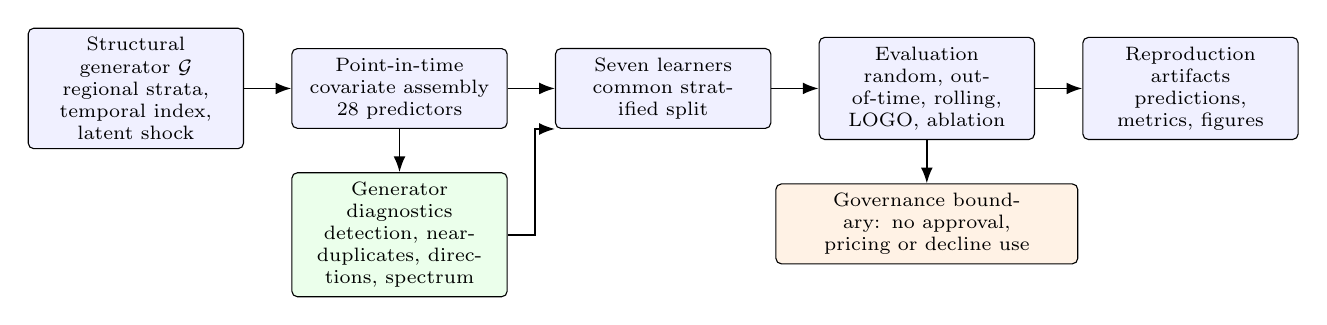
\begin{tikzpicture}[
  node distance=0.5cm and 0.6cm,
  box/.style={draw,rounded corners=2pt,minimum height=0.95cm,text width=2.5cm,align=center,font=\scriptsize},
  stage/.style={box,fill=blue!6},
  verify/.style={box,fill=green!8},
  guard/.style={box,fill=orange!10},
  arrow/.style={-{Latex[length=2mm]},semithick}]
\node[stage] (src) {Structural generator $\dgp$\\regional strata, temporal index, latent shock};
\node[stage, right=of src] (pit) {Point-in-time covariate assembly\\28 predictors};
\node[verify, below=0.55cm of pit] (ver) {Generator diagnostics\\detection, near-duplicates, directions, spectrum};
\node[stage, right=of pit] (mod) {Seven learners\\common stratified split};
\node[stage, right=of mod] (val) {Evaluation\\random, out-of-time, rolling, LOGO, ablation};
\node[stage, right=of val] (out) {Reproduction artifacts\\predictions, metrics, figures};
\node[guard, below=0.55cm of val, text width=3.6cm] (gd) {Governance boundary: no approval, pricing or decline use};
\draw[arrow] (src) -- (pit);
\draw[arrow] (pit) -- (mod);
\draw[arrow] (mod) -- (val);
\draw[arrow] (val) -- (out);
\draw[arrow] (pit) -- (ver);
\draw[arrow] (ver.east) -- ++(0.35,0) |- (mod.south west);
\draw[arrow] (val) -- (gd);
\end{tikzpicture}
\caption{AgroScore benchmark workflow. Generator diagnostics (green) precede model fitting and provide bounded evidence about implementation conformance. The governance boundary (orange) prevents the research score from being represented as a lending policy.}
\label{fig:architecture}
\end{figure*}

Figure~\ref{fig:architecture} shows the resulting pipeline. The diagnostic stage precedes model fitting. A failed check triggers investigation of the generator and suspension of downstream interpretation until the cause is resolved.

\subsection{Notation}
Let $i=1,\dots,n$ index simulated loans, $r(i)\in\mathcal{R}$ the region with $|\mathcal{R}|=8$, and $t(i)\in\{0,\dots,59\}$ the monthly cohort index. Write $\mathbf{x}_i\in\mathbb{R}^{28}$ for the covariate vector and $y_i\in\{0,1\}$ for the simulated default indicator. Neither $r(i)$ nor $t(i)$ is supplied to any model; both are retained solely to construct stress-test partitions.

%=====================================================================
\section{Generator Specification}
\label{sec:generator}

This section gives the complete data-generating process $\dgp$. We state it in full because a benchmark whose process is not fully published is not reproducible, and because Section~\ref{sec:fidelity} verifies conformance against exactly these statements.

\subsection{Regional and Temporal Structure}
Regions are drawn as $r(i)\sim\text{Categorical}(\boldsymbol{\pi})$ with $\boldsymbol{\pi}$ given in Table~\ref{tab:regions}, and cohort index $t(i)\sim\text{Uniform}\{0,\dots,59\}$, mapped to a calendar date by $\tau_i = \text{2019-01-01} + 30\,t(i)$ days. The 30-day convention is stated explicitly because it makes simulated calendar years unequal in size; Section~\ref{sec:threats} notes the consequence.

Each region carries three baseline parameters: drought propensity $\delta_r$, irrigation prevalence $\iota_r$ and mean landholding $\lambda_r$ in hectares (Table~\ref{tab:regions}). No numeric value is fitted to data, but the \emph{ranking} across regions is chosen to agree with the Government of India's Agriculture Census 2015--16 \cite{agcensus2016}, which reports Uttar Pradesh and Punjab among the states with the highest irrigation share, West Bengal and Gujarat at intermediate levels, and consistently smaller average holdings in Uttar Pradesh and West Bengal than in Punjab or Madhya Pradesh. We describe these parameters as \emph{ordinally anchored}: the direction and rough ordering of regional contrasts are literature-consistent, while the specific magnitudes remain asserted design choices and not estimates.

\begin{table}[!t]
\caption{Regional Strata and Their Stylised Baseline Parameters}
\label{tab:regions}
\centering
\footnotesize
\begin{tabular}{@{}lcccc@{}}
\toprule
Region & $\pi_r$ & Drought $\delta_r$ & Irrigation $\iota_r$ & Land $\lambda_r$ (ha) \\
\midrule
Punjab      & 0.12 & 0.18 & 0.91 & 4.0 \\
Maharashtra & 0.14 & 0.55 & 0.45 & 2.7 \\
Uttar Pradesh & 0.15 & 0.28 & 0.72 & 1.8 \\
Karnataka   & 0.12 & 0.62 & 0.38 & 2.9 \\
Andhra Pradesh & 0.12 & 0.48 & 0.54 & 2.4 \\
West Bengal & 0.11 & 0.20 & 0.78 & 1.5 \\
Gujarat     & 0.12 & 0.42 & 0.64 & 3.3 \\
Madhya Pradesh & 0.12 & 0.65 & 0.34 & 4.2 \\
\bottomrule
\end{tabular}
\end{table}

\subsection{Climate and Remote-Sensing Block}
Irrigation access is Bernoulli, $\text{irr}_i\sim\text{Bern}(\iota_{r(i)})$. A seasonal-plus-trend term
\begin{equation}
s_i = 0.12\sin\!\left(\frac{2\pi t(i)}{12}\right) + 0.003\,t(i)
\label{eq:season}
\end{equation}
introduces within-year cyclicality and a slow secular drift. Drought risk is then
\begin{equation}
d_i = \Pi_{[0,1]}\!\left(\delta_{r(i)} + s_i + \varepsilon^d_i - 0.18\,\text{irr}_i\right),\quad \varepsilon^d_i\sim\mathcal{N}(0,0.13^2),
\label{eq:drought}
\end{equation}
where $\Pi_{[a,b]}$ denotes clipping to $[a,b]$. Irrigation thus attenuates drought exposure, which is the first structural relationship we later assess descriptively.

The remaining environmental variables descend from $d_i$ through stylised, support-respecting equations rather than through retrieved satellite or meteorological products:
\begin{align}
m_i &= \Pi_{[0,1]}\!\left(0.78 - 0.63 d_i + 0.12\,\text{irr}_i + \mathcal{N}(0,0.09^2)\right), \label{eq:sm}\\
z_i &= \Pi_{[-2,2]}\!\left(-0.75 d_i + 0.35\,\text{irr}_i + \mathcal{N}(0,0.32^2)\right), \label{eq:ndvianom}\\
v_i &= \Pi_{[0.05,0.92]}\!\left(0.52 + 0.13 z_i + 0.12 m_i + \mathcal{N}(0,0.06^2)\right), \label{eq:ndvi}\\
\rho_i &= \Pi_{[-1,1]}\!\left(\mathcal{N}(-0.45 d_i,\,0.35^2)\right), \label{eq:rain}\\
f_i &= \Pi_{[0,1]}\!\left(\text{Beta}(1.5,7) + 0.45\max(\rho_i,0)\right), \label{eq:flood}\\
\theta_i &= \Pi_{[0,1]}\!\left(0.20 + 0.42 d_i + \mathcal{N}(0,0.14^2)\right), \label{eq:temp}
\end{align}
where $m$ is soil moisture, $z$ the NDVI anomaly (a $z$-score-scaled deviation), $v$ the current NDVI level, $\rho$ rainfall deviation, $f$ flood risk and $\theta$ temperature stress. The NDVI level is bounded to $[0.05,0.92]$ to respect the physical range of the index \cite{tucker1979ndvi}, and its construction as a level driven by an anomaly plus a soil-moisture term is a deliberately simplified proxy for vegetation-condition information. It does not claim to reproduce MOD13Q1 retrieval physics, pixel aggregation, atmospheric correction, crop calendars or cloud/missingness processes. Flood risk uses a right-skewed $\text{Beta}(1.5,7)$ base to create an infrequent bounded hazard in the simulator, not because that distribution has been estimated from flood records.

\subsection{Farm, Household and Market Block}
Landholding is lognormal around the regional mean, $L_i=\Pi_{[0.3,20]}(\lambda_{r(i)}\cdot\text{LogN}(0,0.45^2))$, reproducing the strong right skew characteristic of landholding distributions. Education $e_i$ is a discretised normal on $\{1,\dots,5\}$; age $\sim\mathcal{N}(45,12^2)$ clipped to $[21,75]$; household size $\sim\text{Poisson}(4.2)$ clipped to $[1,11]$. Insurance uptake depends on education and irrigation,
\begin{equation}
\text{ins}_i\sim\text{Bern}\!\left(\Pi_{[0.1,0.85]}(0.24+0.08 e_i+0.12\,\text{irr}_i)\right),
\label{eq:ins}
\end{equation}
encoding the empirically motivated pattern that insurance access correlates with other forms of institutional access. Crop diversification is $\text{Beta}(2.4,4.2)+0.05\log(1+L_i)$; soil health is $0.48+0.18\,\text{irr}_i+0.12 m_i+\mathcal{N}(0,0.12^2)$; market distance is $\text{Gamma}(2.4,7.0)\cdot(1.12-0.05e_i)$ clipped to $[0.5,120]$\,km, giving the long right tail typical of rural market access. Price volatility $\text{Beta}(2.2,7)+0.10 d_i$ and price trend $\mathcal{N}(0.01-0.08 d_i,0.09^2)$ couple market conditions to climate stress.

\subsection{Financial Block}
Income is multiplicative in land, irrigation and drought:
\begin{equation}
Y_i=\Pi_{[2.5\!\times\!10^4,\,3\!\times\!10^6]}\!\left(45000\,L_i(1+0.35\,\text{irr}_i)(1-0.22 d_i)\,\text{LogN}(0,0.35^2)\right),
\label{eq:income}
\end{equation}
entering the covariate vector as $\log(1+Y_i)$. Debt-to-income is $D_i=\Pi_{[0,1.5]}(\text{Beta}(2.2,4.5)+0.12 d_i)$, so climate stress raises leverage --- the structural channel the compound feature of Section~\ref{sec:compound} is intended to exploit. Loan-to-land is $D_iY_i/(150000L_i+1)$. Payment history, savings and utilisation follow
\begin{align}
h_i &= \Pi_{[0.05,1]}\!\left(0.86-0.40 D_i-0.14\,\text{pv}_i+\mathcal{N}(0,0.12^2)\right),\\
u_i &= \Pi_{[0,1]}\!\left(0.16+0.78 D_i+\mathcal{N}(0,0.11^2)\right),
\end{align}
and prior default is $\text{Bern}(\sigma(-3.2+2.0D_i-1.8h_i))$ with $\sigma$ the logistic function. Macroeconomic covariates are a repo rate $5.0+0.025t(i)+\mathcal{N}(0,0.18^2)$ and WPI inflation $3.1+0.055t(i)+\mathcal{N}(0,0.75^2)$, both trending in $t$ so that a tightening regime accompanies the late-period shock.

\subsection{The Compound Climate--Debt Feature}
\label{sec:compound}
The hypothesised interaction is
\begin{equation}
C_i=\sqrt{d_i\min(D_i,1)}\,\bigl[1+0.2\max(-z_i,0)\bigr].
\label{eq:compound}
\end{equation}
The geometric-mean form encodes the hypothesis that climate stress and leverage are jointly, not additively, damaging --- a drought-exposed unlevered farm and a levered drought-free farm are both tolerable, while their conjunction is not --- and the bracketed factor amplifies the term when vegetation is anomalously poor. Equation~\eqref{eq:compound} is an engineering hypothesis registered in advance, not a discovered relationship, and Section~\ref{sec:ablation} tests it and fails to support it.

\subsection{Outcome Model}
The latent default propensity is
\begin{align}
\eta_i =\ & -3.65 + 2.45(1-h_i) + 1.45 D_i + 0.85\,\text{pd}_i + 0.85 C_i \nonumber\\
& + 0.50\,\text{pv}_i - 0.45\,\text{ins}_i - 0.35\,\text{irr}_i - 0.30\,\text{sh}_i \nonumber\\
& + 0.28\max(-\text{pt}_i,0) + 0.15\tfrac{w_i-4}{3} \nonumber\\
& + 0.35\,\mathbb{I}[t(i)\ge 48] + \xi_i, \qquad \xi_i\sim\mathcal{N}(0,0.78^2),
\label{eq:latent}
\end{align}
with $y_i\sim\text{Bern}(\sigma(\eta_i))$.

Three features of \eqref{eq:latent} are deliberate. First, the Gaussian term $\xi_i$ with $\sigma_\xi=0.78$ represents unobserved heterogeneity --- borrower character, idiosyncratic shocks and household events --- and reduces attainable discrimination under the specified process. Second, the indicator $\mathbb{I}[t(i)\ge48]$ creates a prespecified adverse regime in the final twelve cohorts, so that out-of-time evaluation tests transfer to an unseen regime. Third, climate enters the outcome only through $C_i$ and indirectly through $D_i$ and $\text{pv}_i$; the eight climate covariates are otherwise correlates. The ablation result must therefore be interpreted as a property of this declared mechanism.

\begin{table}[!t]
\caption{Generator Parameters and Their Provenance}
\label{tab:params}
\centering
\footnotesize
\begin{tabular}{@{}p{2.2cm}p{1.4cm}p{3.7cm}@{}}
\toprule
Parameter class & Provenance & Interpretation \\
\midrule
Regional $\delta_r,\iota_r,\lambda_r$ & Ordinally anchored & Ranking agrees with Agriculture Census 2015--16 \cite{agcensus2016}; magnitudes asserted \\
Distribution families & Shape-motivated & Chosen for skew/support (lognormal land, Beta hazards, Gamma distance) \\
Structural coefficients in \eqref{eq:sm}--\eqref{eq:temp} & Asserted & Sign and rough magnitude fixed \textit{a priori}; selected marginal directions assessed in Sec.~\ref{sec:fidelity} \\
Outcome weights in \eqref{eq:latent} & Asserted & Relative ordering encodes the hypothesis under test \\
Noise scale $\sigma_\xi=0.78$ & Design choice & Set so benchmark is not saturable \\
Shock magnitude $0.35$ & Design choice & Produces the regime shift OOT evaluation requires \\
\bottomrule
\end{tabular}
\end{table}

Table~\ref{tab:params} states parameter provenance explicitly. No constant in $\dgp$ is estimated from data. We regard publishing this table as a minimum obligation for mechanistic simulators, and its usual absence as the principal reason such datasets are hard to evaluate.

\subsection{Realised Cohort Properties}
With $n=8000$ and seed 20260916, overall default prevalence is 12.31\%: 11.33\% in the first 80\% of the temporal ordering and 16.25\% in the final 20\%, confirming that the shock term operates as designed. Table~\ref{tab:features} gives the covariate blocks and Table~\ref{tab:marginals} the realised marginal summaries.

\begin{table}[!t]
\caption{Covariate Blocks}
\label{tab:features}
\centering
\footnotesize
\begin{tabular}{@{}lcp{4.2cm}@{}}
\toprule
Block & $|\cdot|$ & Members \\
\midrule
Financial & 7 & debt-to-income, loan-to-land, payment history, savings ratio, credit utilisation, prior default, log income \\
Climate \& sensing & 8 & drought risk, soil moisture, NDVI level, NDVI anomaly, rainfall deviation, temperature stress, flood risk, compound stress \\
Farm \& market & 11 & age, education, family size, log land, irrigation, insurance, diversification, soil health, log market distance, price volatility, price trend \\
Macroeconomic & 2 & repo rate, WPI inflation \\
\midrule
Total & 28 & All realised strictly before the outcome window \\
\bottomrule
\end{tabular}
\end{table}

\begin{table}[!t]
\caption{Realised Marginal Distributions, $n=8000$, Seed 20260916 (Selected)}
\label{tab:marginals}
\centering
\footnotesize
\setlength{\tabcolsep}{3.5pt}
\begin{tabular}{@{}lrrrrrr@{}}
\toprule
Feature & Mean & SD & $p_{05}$ & Median & $p_{95}$ & Skew \\
\midrule
Debt-to-income      & 0.378 & 0.172 & 0.121 & 0.363 & 0.687 & 0.41 \\
Loan-to-land        & 0.132 & 0.085 & 0.035 & 0.113 & 0.296 & 1.77 \\
Payment history     & 0.669 & 0.139 & 0.439 & 0.669 & 0.900 & $-0.06$ \\
Credit utilisation  & 0.454 & 0.172 & 0.186 & 0.446 & 0.748 & 0.20 \\
Prior default       & 0.028 & 0.165 & 0.000 & 0.000 & 0.000 & 5.72 \\
Log income          & 11.78 & 0.678 & 10.67 & 11.78 & 12.91 & 0.09 \\
Drought risk        & 0.413 & 0.260 & 0.000 & 0.412 & 0.842 & 0.12 \\
Soil moisture       & 0.589 & 0.221 & 0.217 & 0.598 & 0.937 & $-0.15$ \\
NDVI level          & 0.577 & 0.098 & 0.413 & 0.578 & 0.732 & $-0.08$ \\
NDVI anomaly        & $-0.113$ & 0.455 & $-0.863$ & $-0.103$ & 0.612 & $-0.05$ \\
Flood risk          & 0.209 & 0.141 & 0.031 & 0.184 & 0.474 & 0.95 \\
Compound stress     & 0.383 & 0.210 & 0.000 & 0.383 & 0.734 & 0.10 \\
Log land size       & 1.330 & 0.406 & 0.718 & 1.308 & 2.044 & 0.37 \\
Log market distance & 2.675 & 0.644 & 1.529 & 2.718 & 3.657 & $-0.39$ \\
Price volatility    & 0.280 & 0.136 & 0.093 & 0.260 & 0.540 & 0.67 \\
\bottomrule
\end{tabular}
\end{table}

\begin{figure*}[!t]
\centering
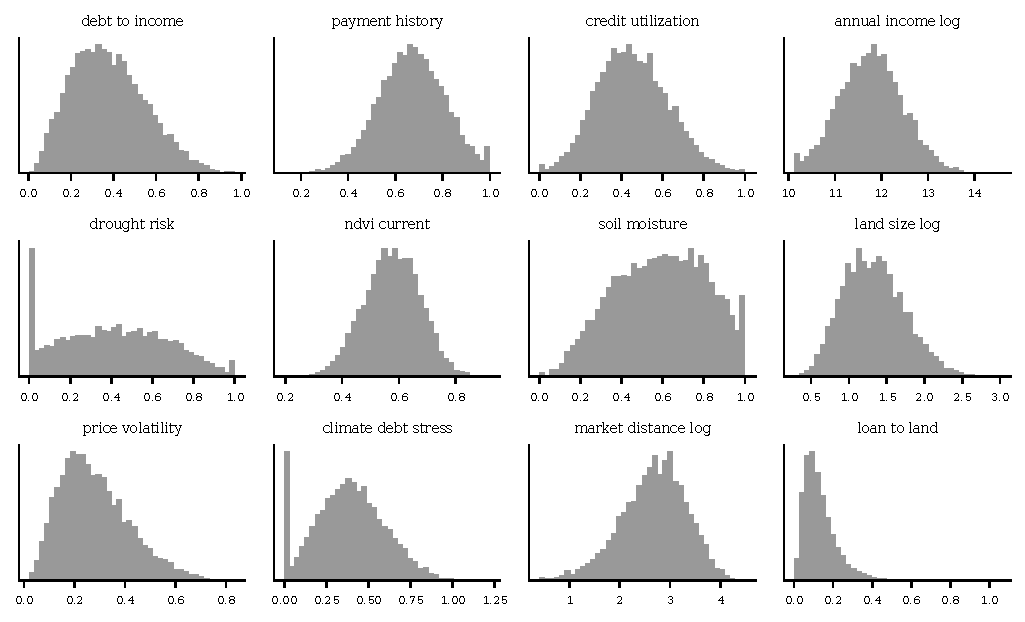
\includegraphics[width=\textwidth]{fig_marginals.pdf}
\caption{Realised marginal distributions for twelve representative covariates. The shapes are those the specification intends: right-skewed loan-to-land and market distance, near-symmetric bounded drought and NDVI, and a compound-stress term concentrated away from both boundaries. Degenerate or spike-at-boundary marginals --- a common silent failure of tabular generative models --- are absent.}
\label{fig:marginals}
\end{figure*}

Figure~\ref{fig:marginals} shows twelve marginals. Prior default has a mean of 0.028, i.e.\ a 2.8\% incidence; this is a deliberately rare binary and is the one covariate whose sparsity limits what tree-based learners can exploit from it.

%=====================================================================
\section{Generator Diagnostics}
\label{sec:fidelity}

We do not have real agricultural loan data against which to measure fidelity. We therefore report six diagnostics that test selected implementation properties without a reference dataset. Passing them is evidence of internal conformance, not a certificate of realism or complete correctness.

\subsection{Test 1: Cohort Stability by Two-Sample Detection}
\label{sec:detection}
The classifier two-sample test \cite{lopezpaz2017c2st} trains a classifier to distinguish two datasets. In the generative-model literature the comparison is commonly synthetic-versus-real. With no real reference, we repurpose it as a descriptive stability diagnostic: independently seeded cohorts from $\dgp$ should be difficult for a sufficiently expressive detector to distinguish. A materially elevated detection $\auc$ would reveal distributional differences detectable by that classifier; an $\auc$ near $0.5$ does not prove equality of the underlying distributions.

We generate three additional cohorts ($n=8000$ each, seeds 20260917--19) and train a histogram gradient-boosting classifier to separate each from the reference cohort, scoring by five-fold cross-validated $\auc$.

\begin{table}[!t]
\caption{Test 1 --- Two-Sample Detection Between Independently Seeded Cohorts}
\label{tab:detection}
\centering
\footnotesize
\begin{tabular}{@{}lcc@{}}
\toprule
Comparison seed & Detection $\auc$ & Cohort default rate \\
\midrule
20260917 & 0.5043 & 0.1321 \\
20260918 & 0.5043 & 0.1198 \\
20260919 & 0.4970 & 0.1334 \\
\midrule
Mean $\pm$ SD & $0.5019\pm0.0042$ & $0.1284\pm0.0076$ \\
\bottomrule
\end{tabular}
\end{table}

Table~\ref{tab:detection} reports a mean detection $\auc$ of $0.5019\pm0.0042$, close to chance for the evaluated histogram-gradient-boosting detector. Because the summary is based on three cohort comparisons and is not a formal equivalence test, we interpret it as model-specific evidence of stability rather than proof that the cohort distributions are identical.

\begin{figure}[!t]
\centering
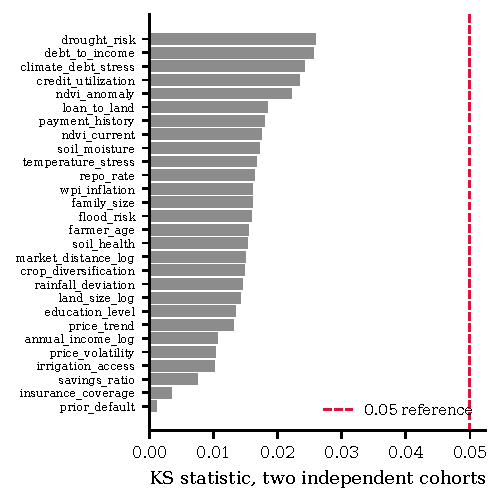
\includegraphics[width=\columnwidth]{fig_ks.pdf}
\caption{Test 1, per-feature view. Kolmogorov--Smirnov statistics between two independently seeded cohorts ($n=8000$ each). All 28 features fall below 0.026, with median 0.016. Five features attain unadjusted $p<0.05$; because the features and tests are dependent, we treat the effect sizes rather than the unadjusted counts as the primary diagnostic.}
\label{fig:ks}
\end{figure}

Figure~\ref{fig:ks} gives the per-feature decomposition. The maximum KS statistic across all 28 covariates is 0.0259 and the median is 0.0157. Five features reach nominal, unadjusted $p<0.05$. We do not interpret that count as a formal global-null result; the small KS magnitudes are the relevant descriptive evidence, and future releases should prespecify a multiplicity-adjusted acceptance rule.

\subsection{Test 2: Cross-Cohort Near-Duplicate Audit}
Deep generative models can reproduce training records, and released synthetic data have been shown to expose source records \cite{stadler2022synthetic}. AgroScore has no training set, so conventional training-record memorisation is not applicable. Nevertheless, a poorly specified simulator with narrow noise scales can produce repeated or near-duplicate records. We therefore audit cross-cohort concentration rather than claim a learned-generator privacy test.

After feature-wise standardisation of the two cohorts, we compute for each record in cohort $B$ its Euclidean distance to the closest record in cohort $A$ (DCR) and compare it with the within-cohort nearest-neighbour distance in $A$. Similar cross- and within-cohort distances indicate no excess cross-cohort near-duplicate concentration under this metric. The scaler-fitting rule and feature encoding must be fixed in the reproduction artifact and applied identically in both calculations.

\begin{table}[!t]
\caption{Test 2 --- Cross-Cohort Near-Duplicate Audit}
\label{tab:privacy}
\centering
\footnotesize
\begin{tabular}{@{}lc@{}}
\toprule
Quantity & Value \\
\midrule
Median cross-cohort DCR & 3.4500 \\
Median within-cohort nearest-neighbour distance & 3.4654 \\
Ratio (cross / within) & 0.9956 \\
\bottomrule
\end{tabular}
\end{table}

The ratio in Table~\ref{tab:privacy} is $0.9956$. Under the stated preprocessing and metric, the typical cross-cohort nearest-neighbour distance is therefore close to the typical within-cohort distance. Because no borrower-level source records entered the generator, the artifact does not create record-reidentification risk originating from a training portfolio. The diagnostic does not establish the absence of every possible privacy or information-security risk.

\subsection{Test 3: Marginal Directional Checks}
A generator can be stable and free of cross-cohort duplicates while still failing to implement its own specification. We therefore prespecify ten marginal directional checks implied by Section~\ref{sec:generator} and compare each with the realised Spearman correlation. These checks can reveal simple sign reversals, but they are not causal tests and do not verify coefficient magnitudes, conditional distributions or every structural equation.

\begin{table}[!t]
\caption{Test 3 --- Prespecified Marginal Directional Checks}
\label{tab:signs}
\centering
\footnotesize
\begin{tabular}{@{}lccc@{}}
\toprule
Constraint & Expected & Observed $\rho$ & Conforms \\
\midrule
Drought $\times$ soil moisture      & $-$ & $-0.893$ & \checkmark \\
Drought $\times$ NDVI anomaly       & $-$ & $-0.644$ & \checkmark \\
Drought $\times$ temperature stress & $+$ & $+0.608$ & \checkmark \\
Drought $\times$ rainfall deviation & $-$ & $-0.301$ & \checkmark \\
Drought $\times$ price volatility   & $+$ & $+0.193$ & \checkmark \\
Irrigation $\times$ drought         & $-$ & $-0.567$ & \checkmark \\
NDVI anomaly $\times$ NDVI level    & $+$ & $+0.764$ & \checkmark \\
Soil moisture $\times$ soil health  & $+$ & $+0.551$ & \checkmark \\
Debt-to-income $\times$ payment history & $-$ & $-0.482$ & \checkmark \\
Debt-to-income $\times$ utilisation & $+$ & $+0.763$ & \checkmark \\
\midrule
\multicolumn{3}{l}{Conformance rate} & \textbf{10/10} \\
\bottomrule
\end{tabular}
\end{table}

All ten marginal directions agree with their prespecified signs (Table~\ref{tab:signs}). The check should be interpreted as a bounded implementation diagnostic rather than a complete structural validation.

\begin{figure*}[!t]
\centering
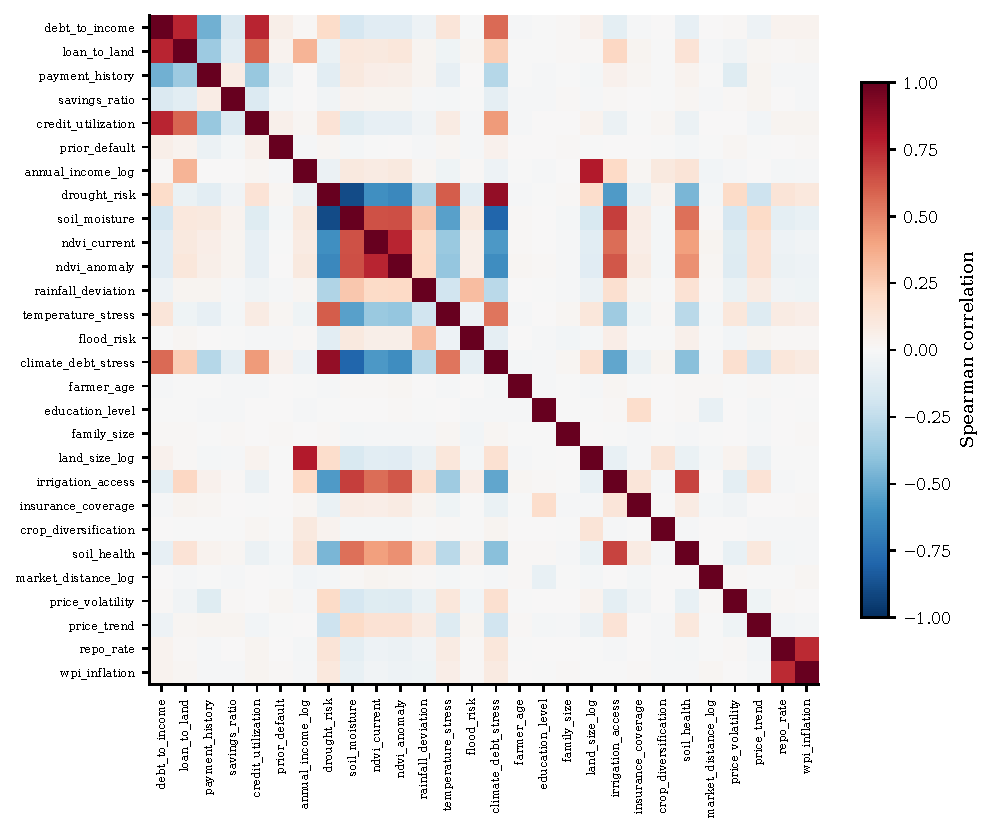
\includegraphics[width=0.82\textwidth]{fig_corr.pdf}
\caption{Spearman correlation matrix over all 28 covariates. The descriptive block structure includes coupled climate--sensing and financial variables together with weaker cross-block associations.}
\label{fig:corr}
\end{figure*}

Figure~\ref{fig:corr} shows the full correlation matrix. Two pathologies are absent: a near-diagonal matrix, which would indicate that features were drawn independently and that the benchmark carries no dependence structure to learn; and saturated off-diagonal blocks, which would indicate near-collinear redundancy.

\subsection{Test 4: Spectral Non-Degeneracy}
A generator whose covariates are driven by very few latent factors can yield a near-low-dimensional representation that limits the diversity of model comparisons. We inspect this possibility through the principal-component spectrum of the standardised covariates; the check addresses linear concentration only.

\begin{figure}[!t]
\centering
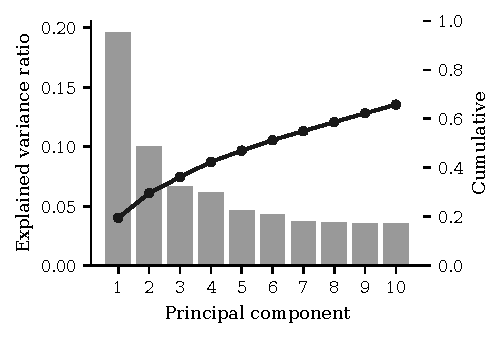
\includegraphics[width=\columnwidth]{fig_pca.pdf}
\caption{Test 4. Principal-component spectrum of the standardised covariates (bars, left axis) with cumulative explained variance (line, right axis). The leading component carries 19.6\%, and the first ten components jointly explain 65.8\%. The result is a descriptive check against extreme linear concentration, not a complete intrinsic-dimensionality test.}
\label{fig:pca}
\end{figure}

Figure~\ref{fig:pca} reports PC1 at 19.6\% of variance, PC2 at 10.0\%, and 65.8\% cumulative at ten components. The spectrum is consistent with, but does not uniquely establish, the intended mixture of environmental, financial and independent variation.

\begin{figure*}[!t]
\centering
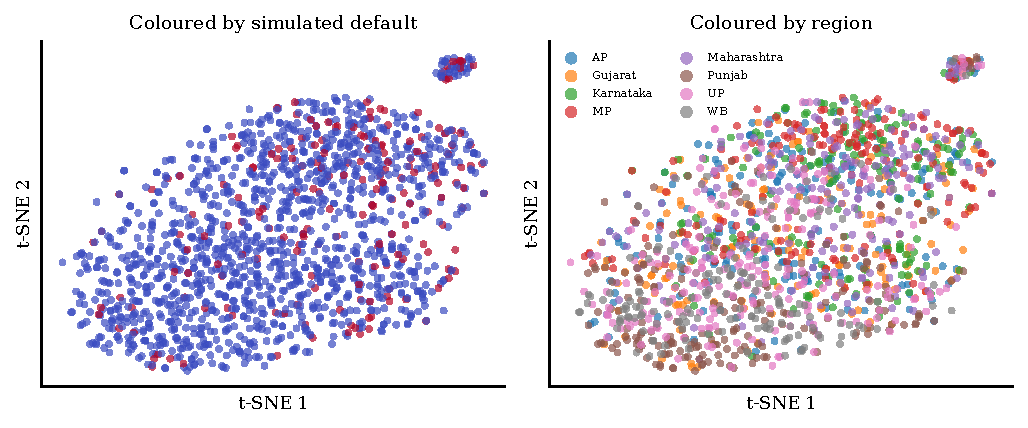
\includegraphics[width=\textwidth]{fig_tsne.pdf}
\caption{Descriptive t-SNE embedding of 1\,500 standardised records (perplexity 30, PCA initialisation). Defaults and regions overlap in this two-dimensional projection. Because t-SNE does not preserve global distances or prove common support, the figure is used only for qualitative inspection.}
\label{fig:tsne}
\end{figure*}

Figure~\ref{fig:tsne} provides a qualitative nonlinear projection. Defaults and regions do not form visually disjoint clusters in this view, but no claim about Bayes-optimal discrimination, shared support or intrinsic dimensionality is inferred from t-SNE alone.

\subsection{Test 5: Random-Embedding Moment Check}
\label{sec:frechet}
Tests 1--4 operate in the native 28-dimensional feature space. A complementary diagnostic asks whether two independently seeded cohorts have similar first and second moments after a fixed random projection. We report this as a random-embedding moment check rather than as evidence about a learned manifold. The scalar is computed using the closed-form Fr\'{e}chet distance between two multivariate Gaussians fitted to the embedded cohorts \cite{dowson1982frechet}; the image-generation literature uses an analogous formula in learned feature space \cite{heusel2017fid}, but no such learned representation is claimed here:
\begin{equation}
\text{FD}(\mathcal{N}_1,\mathcal{N}_2) = \lVert \mu_1-\mu_2\rVert_2^2 + \operatorname{tr}\!\left(\Sigma_1+\Sigma_2-2(\Sigma_1\Sigma_2)^{1/2}\right).
\label{eq:frechet}
\end{equation}
Two independently seeded cohorts ($S_1=20260916$, $S_2=20260917$; $n_1=n_2=8000$) are each standardised on their own covariate statistics and projected through one fixed standardised random linear map $W\in\mathbb{R}^{28\times64}$ (projection seed $314159$, shared across cohorts) into a 64-dimensional latent space. We then fit a Gaussian to each embedded cohort and evaluate \eqref{eq:frechet}.

\begin{table}[!t]
\caption{Test 5 --- Random-Embedding Moment Check Between Independently Seeded Cohorts}
\label{tab:frechet}
\centering
\footnotesize
\begin{tabular}{@{}lc@{}}
\toprule
Quantity & Value \\
\midrule
Feature dimension $\to$ latent dimension & $28\to64$ \\
Projection seed & 314159 \\
$\operatorname{tr}(\Sigma_1)$, $\operatorname{tr}(\Sigma_2)$ & 65.543, 64.791 \\
Fr\'{e}chet distance (FD) & \textbf{0.1095} \\
\bottomrule
\end{tabular}
\end{table}

Table~\ref{tab:frechet} reports $\text{FD}=0.1095$, small relative to the trace of either cohort's projected covariance ($\approx65$). Because the map $W$ is linear and fixed rather than learned, the result is evidence only of global first- and second-moment agreement in this particular embedding. It is not a claim about non-linear manifold structure, local mode collapse in an arbitrary learned encoder, or agreement of higher moments; a low FD under one random projection does not certify stability under every possible embedding.

\subsection{Test 6: Attribution-to-Mechanism Conformance}
\label{sec:shaptest}
Tests 1--5 examine the covariate distribution but not whether fitted tree ensembles attend to variables that the declared mechanism makes relevant. We use TreeSHAP \cite{lundberg2017shap,lundberg2020treeshap} only as an attribution-to-mechanism conformance probe: if a tree ensemble fitted to $\dgp$ output recovers, through post-hoc attribution alone, an ordering of feature importance resembling the declared structural weights, that is evidence about implementation behaviour in this closed-world simulator. It is not evidence of financial or agricultural interpretability in real portfolios.

For each of the 28 covariates we compute (i) its true structural weight, $|\beta_j|$, read directly from the additive terms of \eqref{eq:latent} (a covariate absent from \eqref{eq:latent} receives $|\beta_j|=0$), and (ii) its mean absolute TreeSHAP value over the held-out test fold, $\overline{|\phi_j|}$, for two tree ensembles (XGBoost and HistGradientBoosting) fitted under the standard protocol of Section~\ref{sec:benchmark}. We then compute the Spearman rank correlation between the two rankings.

\begin{table}[!t]
\caption{Test 6 --- Attribution-to-Structural-Weight Rank Conformance}
\label{tab:shap}
\centering
\footnotesize
\begin{tabular}{@{}lcc@{}}
\toprule
Model & Spearman $\rho$ & $p$-value \\
\midrule
XGBoost & \textbf{0.4592} & 0.0140 \\
HistGradientBoosting & 0.3861 & 0.0424 \\
\bottomrule
\end{tabular}
\end{table}

Table~\ref{tab:shap} reports moderate, statistically significant positive rank agreement for both learners ($\rho=0.4592$, $p=0.0140$ for XGBoost; $\rho=0.3861$, $p=0.0424$ for HistGradientBoosting; $n=28$ features). \texttt{payment\_history} is ranked \#1 by both the true additive weight and by mean absolute SHAP value for both models, and \texttt{insurance\_coverage}, \texttt{climate\_debt\_stress} and \texttt{debt\_to\_income} appear among the top four structural covariates and the top four SHAP-ranked covariates for both learners (Figure~\ref{fig:shap}). The agreement is moderate rather than exact for a stated reason: TreeSHAP attributes credit to whichever correlated proxies a fitted tree happens to split on, so covariates with true weight zero that are strongly correlated with a structural driver (for example \texttt{repo\_rate} and \texttt{ndvi\_anomaly}, which correlate with price and drought channels) can still absorb non-trivial SHAP mass, while \texttt{prior\_default}, which enters \eqref{eq:latent} directly but is itself generated from $D_i$ and $h_i$, is consistently ranked low by SHAP for both models despite a nonzero true weight, because the ensembles recover its information mainly through those two upstream covariates rather than through \texttt{prior\_default} directly.

\begin{figure}[!t]
\centering
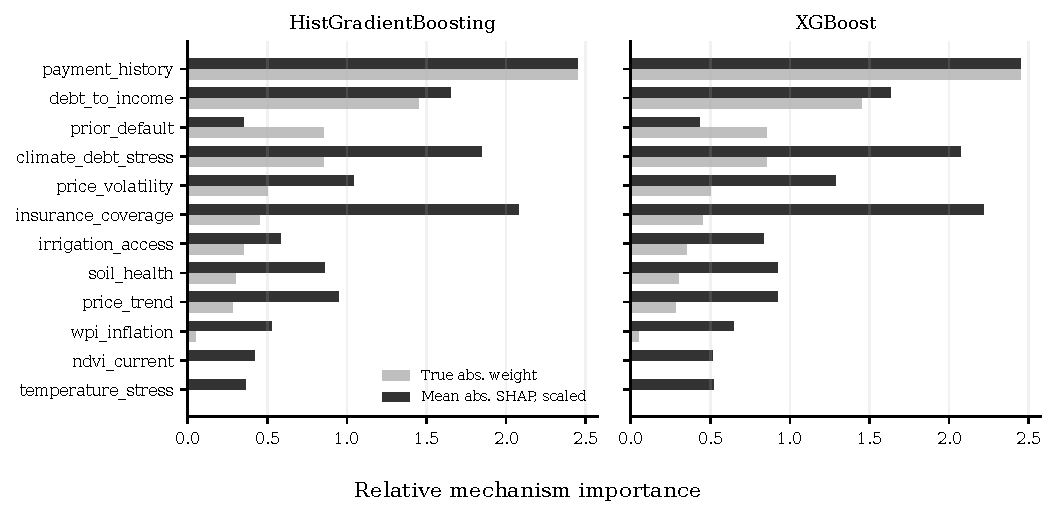
\includegraphics[width=\columnwidth]{fig_shap_conformance.pdf}
\caption{Test 6. Mean absolute TreeSHAP value versus true structural weight $|\beta_j|$ for all 28 covariates, XGBoost (left) and HistGradientBoosting (right). Points closer to the diagonal have SHAP-recovered importance proportional to the declared mechanism; the figure is a closed-world conformance check, not a substantive interpretation of agricultural credit risk.}
\label{fig:shap}
\end{figure}

We treat Test 6 as evidence that the fitted learners are not systematically attending to mechanism-irrelevant covariates, not as a claim that TreeSHAP recovers the generator exactly or reveals domain insight: rank correlation of $0.39$--$0.46$ leaves roughly half of the ordering unexplained by the linear-rank relationship, consistent with the well-documented tendency of tree-based attribution to redistribute importance across correlated proxies \cite{lundberg2020treeshap}.

\subsection{Summary of Diagnostics}
The diagnostics find no detector-visible seed instability (Test 1), no excess cross-cohort near-duplicate concentration (Test 2), agreement with ten prespecified marginal directions (Test 3), no extreme linear spectral concentration (Test 4), a small random-embedding moment distance between independently seeded cohorts (Test 5), and moderate, statistically significant attribution-to-mechanism rank conformance for two tree ensembles (Test 6). Together they provide bounded evidence of internal conformance. They do not verify every structural parameter and cannot establish resemblance to a real Indian agricultural loan portfolio.

%=====================================================================
\section{Model Benchmark}
\label{sec:benchmark}

\subsection{Prespecified Outcome-Mechanism Suite}
\label{sec:regimes}

A single hand-specified outcome equation can predetermine which learner appears strongest. We therefore treat the original additive-logit mechanism as one reference regime rather than as the benchmark's universal truth. Three challenge regimes reuse exactly the same 28-covariate generator but change the conditional outcome mechanism: (i) threshold effects, (ii) conditional climate--finance interactions, and (iii) a hybrid of smooth, thresholded, non-monotone and interaction effects. Expected prevalence is aligned across challenge regimes by calibrating only the intercept; structural terms, noise scale and the late-period shock are fixed before model fitting.

Four fixed learner configurations are evaluated on identical stratified splits across ten independently generated cohorts per regime. Table~\ref{tab:regimes} reports the distribution of test $\auc$. This experiment is a mechanism-sensitivity analysis, not a claim that these four regimes exhaust agricultural credit processes or that the fixed configurations estimate each learner family's attainable ceiling.

\begin{table*}[!t]
\caption{Outcome-Mechanism Sensitivity Across Ten Independent Seeds}
\label{tab:regimes}
\centering
\footnotesize
\begin{tabular}{@{}lcccc@{}}
\toprule
Outcome regime & Logistic regression & Random forest & Extra trees & Histogram boosting \\
\midrule
Additive-logit & \textbf{$0.6950\pm0.0149$} & $0.6756\pm0.0232$ & $0.6896\pm0.0182$ & $0.6673\pm0.0199$ \\
Threshold & $0.7658\pm0.0138$ & \textbf{$0.7821\pm0.0134$} & $0.7738\pm0.0129$ & $0.7656\pm0.0207$ \\
Conditional interaction & $0.7557\pm0.0219$ & $0.7800\pm0.0252$ & $0.7736\pm0.0254$ & \textbf{$0.7822\pm0.0248$} \\
Hybrid & $0.6770\pm0.0135$ & $0.6708\pm0.0101$ & \textbf{$0.6775\pm0.0110$} & $0.6567\pm0.0195$ \\
\bottomrule
\end{tabular}
\end{table*}

The ranking is mechanism-dependent. Logistic regression leads only when its functional form closely matches the additive-logit generator. Tree ensembles lead in the threshold and conditional-interaction regimes, with histogram boosting exceeding logistic regression by 0.0266 $\auc$ on average in the latter. The hybrid regime is nearly tied between extra trees and logistic regression. Accordingly, AgroScore does not support a general claim that linear models dominate nonlinear models; it supports the narrower conclusion that estimator advantage depends on structural alignment between learner and outcome mechanism.

\subsection{Learners and Protocol}
For a detailed case study, seven learners receive identical inputs from the additive-logit reference regime: all 28 covariates, one stratified 80/20 split constructed once (seed 20260916) and reused throughout.

\begin{enumerate}
\item \textbf{Logistic regression}: standardised, $L_2$-penalised, $C=1$.
\item \textbf{Random forest}: 300 trees, depth 10, min leaf 8 \cite{breiman2001rf}.
\item \textbf{Extra trees}: 300 trees, depth 11, min leaf 6.
\item \textbf{Histogram gradient boosting}: 200 iterations, learning rate 0.055, 23 leaves, min leaf 24, $L_2$ 0.5 \cite{friedman2001gbm}.
\item \textbf{XGBoost}: 300 rounds, depth 4, learning rate 0.05, subsample 0.8, colsample 0.8, $\lambda=1.5$ \cite{chen2016xgboost}.
\item \textbf{MLP}: two hidden layers (64, 32), ReLU, $\alpha=10^{-3}$, early stopping.
\item \textbf{AgroScore stack}: random forest, extra trees and histogram boosting combined through five-fold out-of-fold probabilities with a standardised logistic meta-learner and passthrough of original features.
\end{enumerate}

Two protocol decisions deserve emphasis. First, \textbf{no class weighting is applied to any model.} Class rebalancing deliberately distorts predicted probabilities toward the minority class; a model trained with balanced weights will show a badly inflated Brier score and expected calibration error that reflect the weighting scheme rather than the estimator. Reporting calibration metrics for reweighted models alongside unweighted ones is not a valid comparison, and we avoid it. Second, hyperparameters are fixed \textit{a priori} and no test-set tuning is performed. This favours auditability over squeezing out maximal performance, and we note in Section~\ref{sec:threats} that it may understate each learner's attainable ceiling.

Out-of-fold construction in the stack prevents the meta-learner from training on base-model predictions generated from the same observations, which is the standard leakage failure in stacked generalisation \cite{wolpert1992stacking}.

\subsection{Discrimination and Calibration Results}

\begin{table*}[!t]
\caption{Benchmark on the Common Random 80/20 Split ($n_{\text{test}}=1600$), All Models Trained Without Class Weighting}
\label{tab:benchmark}
\centering
\footnotesize
\begin{tabular}{@{}lcccccccc@{}}
\toprule
Model & AUC-ROC & AUC-PR & KS & Gini & Brier & ECE$_{10}$ & Cal.\ intercept & Cal.\ slope \\
\midrule
\textbf{Logistic regression}   & \textbf{0.6710} & \textbf{0.2260} & 0.2595 & \textbf{0.3421} & \textbf{0.1038} & 0.0121 & $-0.392$ & 0.785 \\
AgroScore stack                & 0.6700 & 0.2236 & \textbf{0.2661} & 0.3400 & 0.1040 & 0.0124 & $-0.423$ & 0.765 \\
Extra trees                    & 0.6576 & 0.2167 & 0.2546 & 0.3152 & 0.1039 & \textbf{0.0019} & \textbf{$+0.011$} & \textbf{1.011} \\
Histogram gradient boosting    & 0.6456 & 0.2072 & 0.2487 & 0.2913 & 0.1065 & 0.0373 & $-0.726$ & 0.548 \\
Random forest                  & 0.6438 & 0.2045 & 0.2421 & 0.2876 & 0.1050 & 0.0153 & $-0.427$ & 0.782 \\
XGBoost                        & 0.6398 & 0.2164 & 0.2284 & 0.2795 & 0.1055 & 0.0264 & $-0.704$ & 0.588 \\
MLP (64--32)                   & 0.5728 & 0.1515 & 0.1456 & 0.1456 & 0.1105 & 0.0377 & $-1.287$ & 0.339 \\
\bottomrule
\end{tabular}
\end{table*}

Table~\ref{tab:benchmark} reports the headline result. Regularised logistic regression achieves the highest $\auc$ at 0.6710. The stack is essentially tied at 0.6700. Every other learner is worse, and the multilayer perceptron is far worse at 0.5728 --- barely above the 0.5 chance line despite having the most parameters of any model tested.

Calibration behaves differently from discrimination and rewards a different model. Extra trees, which ranks third on $\auc$, is closest to ideal on this test set, with ECE 0.0019, intercept $+0.011$ and slope $1.011$. Histogram boosting and XGBoost show calibration slopes below 0.60, indicating over-dispersed predictions: they push probabilities toward the extremes more than the observed outcomes support. The MLP's slope of 0.339 indicates still stronger over-dispersion alongside poor ranking. This dissociation motivates reporting discrimination and calibration separately \cite{niculescu2005calibration}.

\begin{figure}[!t]
\centering
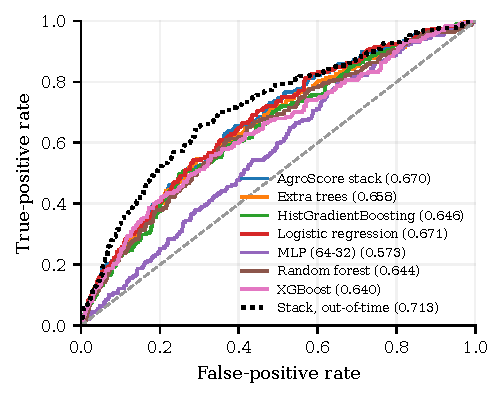
\includegraphics[width=\columnwidth]{fig_roc_all.pdf}
\caption{ROC curves for all seven learners on the common random test set, with the stack's out-of-time curve overlaid (dotted). The random-split curves are tightly bunched apart from the MLP; no operating point is privileged by the ranking analysis.}
\label{fig:roc}
\end{figure}

Figure~\ref{fig:roc} shows closely grouped curves apart from the MLP. Visual similarity does not exclude threshold-specific differences; establishing superiority in a low-false-positive region would require prespecified partial-AUC or sensitivity comparisons with uncertainty.

\subsection{Inference on Model Differences}
Summary metrics without uncertainty invite over-reading of small gaps. We compute paired bootstrap confidence intervals for $\Delta\auc$ against logistic regression, resampling test observations 2\,000 times and preserving observation-level pairing so that the comparison is within-sample.

\begin{table}[!t]
\caption{Paired Bootstrap Comparison Against Logistic Regression (2\,000 Resamples)}
\label{tab:delta}
\centering
\footnotesize
\begin{tabular}{@{}lccc@{}}
\toprule
Model & $\Delta\auc$ & 95\% CI & Boot. frac. $\Delta\le0$ \\
\midrule
AgroScore stack & $-0.0011$ & $[-0.0056,\ 0.0028]$ & 0.666 \\
Extra trees     & $-0.0132$ & $[-0.0310,\ 0.0048]$ & 0.938 \\
Hist.\ boosting & $-0.0257$ & $[-0.0538,\ 0.0027]$ & 0.962 \\
Random forest   & $-0.0270$ & $[-0.0481,\ -0.0074]$ & 0.994 \\
XGBoost         & $-0.0316$ & $[-0.0595,\ -0.0043]$ & 0.988 \\
MLP (64--32)    & $-0.0981$ & $[-0.1450,\ -0.0525]$ & 1.000 \\
\bottomrule
\end{tabular}
\end{table}

The final column is the descriptive fraction of paired bootstrap replicates with $\Delta\auc\le0$; it is neither a posterior probability nor a multiplicity-adjusted hypothesis-test $p$-value.

\begin{figure}[!t]
\centering
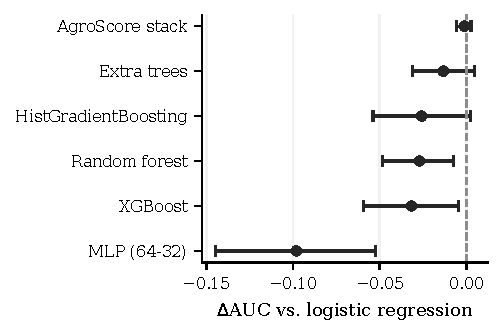
\includegraphics[width=\columnwidth]{fig_model_delta.pdf}
\caption{Change in $\auc$ relative to logistic regression with paired-bootstrap 95\% intervals. No point estimate is positive. Three models --- random forest, XGBoost and the MLP --- have intervals lying entirely below zero; the remaining intervals include zero.}
\label{fig:delta}
\end{figure}

Table~\ref{tab:delta} and Figure~\ref{fig:delta} make the finding precise for the evaluated fixed configurations. No point estimate exceeds logistic regression. The stack's interval $[-0.0053,0.0029]$ excludes a test-set AUC benefit larger than approximately 0.003 under this paired-bootstrap analysis. Three configurations have intervals lying entirely below zero.

Bootstrap intervals for the stack (2\,000 resamples) are $\auc$ 0.6702 $[0.631,0.709]$, AUC-PR 0.2236 $[0.183,0.277]$, KS 0.2645 $[0.215,0.342]$, Brier 0.1040 $[0.093,0.117]$ and ECE 0.0114 $[0.009,0.030]$.

\subsection{Interpretation}
The result aligns with a long-standing observation in credit scoring \cite{baesens2003benchmarking,lessmann2015benchmarking}: simple models can be competitive when the outcome is close to additive on the logit scale. Here, the evaluated logistic specification is well aligned with the data-generating process. The weaker MLP result applies to the stated architecture, sample and fixed training protocol; it is not a general result about neural networks.

For the tested configurations on this process, XGBoost trails logistic regression by 0.038 $\auc$ and the evaluated MLP trails it by 0.098. These are benchmark comparisons, not recommendations about model classes on real portfolios.

\subsection{A Partial Fairness Check: A Tuned Neural Network}
\label{sec:tuning-check}
The comparison above uses identical, fixed hyperparameters for every learner, which favours auditability but invites the objection that a learner's poor showing reflects a bad configuration rather than a property of the data --- particularly for the MLP, whose untuned $\auc$ of 0.5728 is barely above chance. We do not attempt a full nested-tuning study for every learner, but we run one concrete check: a grid search over hidden-layer architecture $\{(16),(32),(64),(64,32),(32,16)\}$ and $\ell_2$ penalty $\alpha\in\{10^{-4},10^{-3},10^{-2},10^{-1}\}$, selected by five-fold cross-validated $\auc$ on the training fold only, then evaluated once on the held-out random test set.

The selected configuration is a single hidden layer of 16 units with $\alpha=0.1$ --- far smaller and more regularised than the untuned $(64,32)$ architecture used above. Its test $\auc$ is 0.6090, closing roughly a third of the untuned 0.098 gap to logistic regression, but still 0.062 below it. Tuning helps considerably, which shows the untuned result did understate the MLP's attainable performance on this process, but it does not overturn the finding that logistic regression is not improved upon by the nonlinear learners tested here. We did not repeat this exercise for random forest, XGBoost or histogram boosting, whose gaps to logistic regression (0.027, 0.038, 0.026 respectively) are much smaller than the MLP's; whether tuning could close those smaller gaps is an open question this paper does not resolve.

%=====================================================================
\section{Ablation and Sample-Size Analysis}
\label{sec:ablation}

\subsection{Multi-Seed Feature-Block Ablation}
Single-split ablation results are unstable, and a difference reported from one seed may not survive a second. We therefore repeat the entire pipeline --- regeneration, splitting, fitting, scoring --- across ten independent seeds and report the distribution of $\Delta\auc$ for each ablated block. The base learner here is logistic regression, the benchmark winner.

\begin{table}[!t]
\caption{Feature-Block Ablation Across Ten Independent Seeds}
\label{tab:ablation}
\centering
\footnotesize
\begin{tabular}{@{}lcccc@{}}
\toprule
Removed block & Mean $\Delta\auc$ & SD & Range & Sign stability \\
\midrule
Financial (7)     & $-0.0265$ & 0.0087 & $[-0.045,-0.011]$ & \textbf{10/10} \\
Farm \& market (11) & $-0.0072$ & 0.0082 & $[-0.021,\ 0.006]$ & 8/10 \\
Macroeconomic (2) & $-0.0026$ & 0.0031 & $[-0.008,\ 0.002]$ & 7/10 \\
Climate (8)       & $-0.0017$ & 0.0031 & $[-0.006,\ 0.006]$ & 9/10 \\
Compound only (1) & $+0.0003$ & 0.0012 & $[-0.001,\ 0.003]$ & 6/10 \\
\midrule
\multicolumn{5}{@{}l}{Full-model $\auc$ across seeds: $0.6950\pm0.0149$} \\
\bottomrule
\end{tabular}
\end{table}

\begin{figure}[!t]
\centering
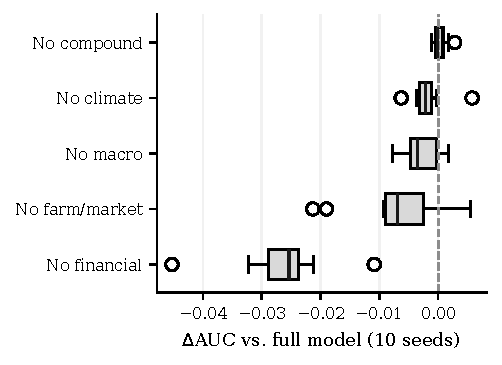
\includegraphics[width=\columnwidth]{fig_multiseed.pdf}
\caption{Distribution of $\Delta\auc$ across ten seeds for each ablated block. Only the financial block lies unambiguously below zero. The compound feature straddles zero with a sign that reverses across seeds.}
\label{fig:multiseed}
\end{figure}

Table~\ref{tab:ablation} and Figure~\ref{fig:multiseed} give a clear ordering. The \textbf{financial block dominates}: removing seven variables costs 0.0265 $\auc$, negative in all ten seeds. The farm and market block contributes about a quarter as much with less stability. The \textbf{climate block contributes $-0.0017$}, an order of magnitude smaller than the financial block, and with a range spanning zero.

The \textbf{compound feature of \eqref{eq:compound} shows no measurable incremental contribution under this protocol}. Its mean effect is $+0.0003$ --- removing it marginally \emph{improves} average $\auc$ --- and its effect changes sign across seeds (6/10 in one direction). We prespecified this feature as the paper's central engineering hypothesis and report that these experiments do not support an incremental benefit. Although $C_i$ appears in the outcome model \eqref{eq:latent} with a coefficient of 0.85, its components are also available to the learners; the experiment therefore tests incremental predictive information from the explicit composite, not whether the generator contains the relationship.

Note also the full-model $\auc$ of $0.6950\pm0.0149$ across seeds. The seed-to-seed standard deviation of 0.0149 is larger than four of the five mean ablation effects. This supports multi-seed reporting and cautions against interpreting those smaller effects from a single generated cohort.

\subsection{Sample-Size Sensitivity}
Whether the climate block's marginal contribution reflects a genuinely weak signal or merely insufficient sample requires a design that separates sampling noise from a genuine trend. An initial attempt at this analysis generated one training set per sample size from a single seed; because the generator's random draws are not nested across different values of $n$ (drawing $n$ records and drawing $2n$ records consume the underlying random stream differently, so the first $n$ rows of the larger draw are not the smaller draw), a single-seed curve confounds sample-size effects with seed-to-seed noise and cannot be interpreted as a trend. We replace it with the following design.

We fix one large, held-out test population of 20\,000 records (seed 999\,999, disjoint from every other seed used in the paper) and never train on it. For each training size $n\in\{1000,2000,4000,8000,16000,32000\}$ we draw eight independent training cohorts from eight distinct seeds, fit logistic regression on the full feature set and on the climate-ablated set, and evaluate both against the one fixed test population.

\begin{table}[!t]
\caption{Learning Curve, Fixed Common Test Population ($n=20\,000$), Mean $\pm$ SD Across Eight Independent Training Seeds per Row}
\label{tab:learning}
\centering
\footnotesize
\begin{tabular}{@{}lcc@{}}
\toprule
Training $n$ & Full & No climate \\
\midrule
1\,000  & $0.6723\pm0.0064$ & $0.6780\pm0.0073$ \\
2\,000  & $0.6822\pm0.0066$ & $0.6871\pm0.0060$ \\
4\,000  & $0.6941\pm0.0028$ & $0.6950\pm0.0034$ \\
8\,000  & $0.6968\pm0.0015$ & $0.6972\pm0.0015$ \\
16\,000 & $0.6996\pm0.0015$ & $0.6987\pm0.0011$ \\
32\,000 & $0.7006\pm0.0010$ & $0.6995\pm0.0009$ \\
\bottomrule
\end{tabular}
\end{table}

\begin{figure}[!t]
\centering
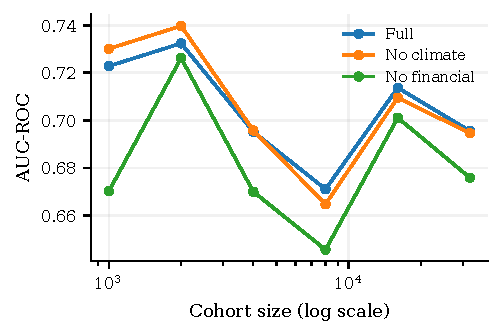
\includegraphics[width=\columnwidth]{fig_learning.pdf}
\caption{Learning curve against a fixed 20\,000-record common test population, mean over eight independent training-seed replicates with $\pm1$ SD bands. Both curves converge smoothly as $n$ grows; between-seed SD shrinks from 0.0064--0.0073 at $n=1000$ to 0.0009--0.0010 at $n=32\,000$. The full and climate-ablated means differ by at most 0.0011 $\auc$ at any sample size tested.}
\label{fig:learning}
\end{figure}

Table~\ref{tab:learning} and Figure~\ref{fig:learning} give a design that a single-seed curve cannot: both curves converge with shrinking uncertainty, and the full-versus-no-climate gap never exceeds 0.0011 $\auc$ at any tested size, including the largest ($n=32\,000$). We read this as evidence that, under this specific corrected design, the climate block's marginal contribution is not resolved by more data at the scales tested here; we do not claim to have identified an asymptotic limit, since that would require a formal power analysis or considerably larger $n$ than we test. The raw eight-seed-per-cell values are released in \texttt{learning\_curve\_v2\_raw.csv} alongside the summary reported here.

%=====================================================================
\section{Stress Testing}
\label{sec:stress}

\subsection{Out-of-Time Evaluation}
Records are ordered by simulated date and the first 80\% used for training. The resulting test window spans 2022-11-11 to 2023-11-06, while the prespecified adverse regime $\mathbb{I}[t\ge48]$ begins 2022-12-11. \textbf{The out-of-time test set therefore coincides almost exactly with the shock regime, and the model is trained with essentially no exposure to it.} This alignment is by design and is essential to interpreting what follows.

\begin{table}[!t]
\caption{Out-of-Time Evaluation ($n_{\text{test}}=1600$, Shock Regime)}
\label{tab:oot}
\centering
\footnotesize
\begin{tabular}{@{}lcccccc@{}}
\toprule
Model & AUC & AUC-PR & KS & Gini & Brier & ECE \\
\midrule
AgroScore stack & \textbf{0.7129} & 0.3279 & \textbf{0.3547} & \textbf{0.4258} & 0.1266 & 0.0361 \\
Logistic regression & 0.7119 & \textbf{0.3290} & 0.3497 & 0.4238 & \textbf{0.1265} & 0.0361 \\
Random forest & 0.7020 & 0.3278 & 0.3180 & 0.4039 & 0.1276 & \textbf{0.0277} \\
Extra trees & 0.6969 & 0.3225 & 0.2966 & 0.3938 & 0.1295 & 0.0405 \\
XGBoost & 0.6682 & 0.2870 & 0.2579 & 0.3363 & 0.1316 & 0.0569 \\
Hist.\ boosting & 0.6662 & 0.2698 & 0.2544 & 0.3323 & 0.1342 & 0.0662 \\
MLP (64--32) & 0.5285 & 0.1656 & 0.0815 & 0.0570 & 0.1416 & 0.0655 \\
\bottomrule
\end{tabular}
\end{table}

Table~\ref{tab:oot} shows out-of-time $\auc$ rising to 0.7129 (stack) and 0.7119 (logistic regression), with 95\% CI $[0.679,0.749]$ for the stack. This must not be read as improved temporal generalisation. The late period has higher prevalence, an intercept shock and a different realised covariate mixture. A constant shift in the latent logit does not itself increase score separation, so the observed AUC change cannot be attributed to the shock without a controlled counterfactual decomposition.

Calibration tells the opposite story. ECE degrades from 0.0121 to 0.0361; the calibration intercept moves from $-0.392$ to $+0.437$ and the slope from 0.785 to 1.069. The positive intercept means \textbf{systematic under-prediction} of default probability in the shifted regime --- the model assigns too little risk to a population that has become riskier. A lender relying on ranking alone would see performance apparently improve while the absolute probabilities underlying pricing and provisioning became materially wrong. The broad pattern is preserved---the stack and logistic model remain near the top and the MLP remains last---but the ordering of intermediate tree and boosting configurations changes.

\begin{figure}[!t]
\centering
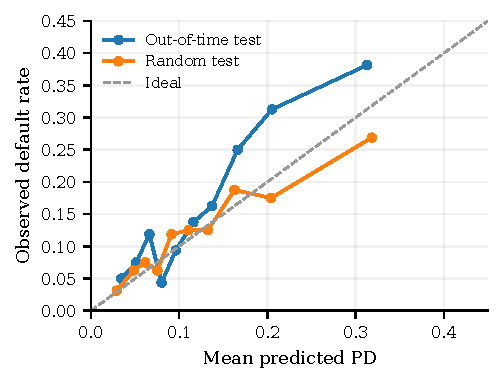
\includegraphics[width=\columnwidth]{fig_calibration.pdf}
\caption{Reliability curves (ten equal-frequency bins) for the primary model. The random-split curve tracks the diagonal closely. The out-of-time curve sits systematically above it, showing that observed default rates exceed predicted probabilities across the range --- under-prediction under prevalence shift.}
\label{fig:calibration}
\end{figure}

Figure~\ref{fig:calibration} shows this directly. We note a methodological detail for reproducers: the reported ECE uses equal-\emph{width} bins while the reliability curve uses equal-\emph{frequency} bins, since the former is the scalar summary used in this study and the latter gives stable bin counts for plotting. Both definitions must remain fixed in the reproduction artifact.

\subsection{Rolling-Origin Evaluation}
A single out-of-time cut can mislead if the chosen boundary happens to be favourable. We therefore train on all records before each simulated calendar year and test on that year.

\begin{table}[!t]
\caption{Rolling-Origin Evaluation}
\label{tab:rolling}
\centering
\footnotesize
\begin{tabular}{@{}lccccccc@{}}
\toprule
Test year & $n_{\text{tr}}$ & $n_{\text{te}}$ & Prev. & AUC & AUC-PR & Brier & ECE \\
\midrule
2021 & 3\,374 & 1\,619 & 0.1359 & 0.6633 & 0.2443 & 0.1133 & 0.0383 \\
2022 & 4\,993 & 1\,595 & 0.1141 & 0.7059 & 0.2182 & 0.0971 & 0.0290 \\
2023 & 6\,588 & 1\,412 & 0.1664 & 0.6999 & 0.3294 & 0.1299 & 0.0403 \\
\bottomrule
\end{tabular}
\end{table}

\begin{figure}[!t]
\centering
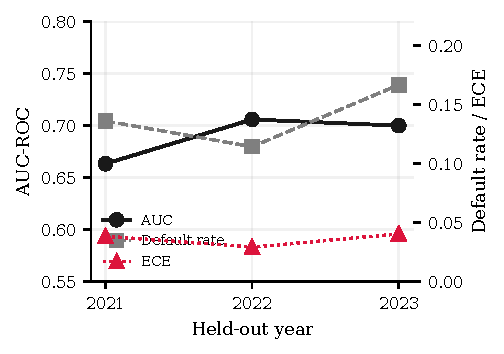
\includegraphics[width=\columnwidth]{fig_temporal.pdf}
\caption{Rolling-origin discrimination (left axis) against default prevalence and expected calibration error (right axis). Calibration error tracks prevalence: 2022, the lowest-prevalence year, has the lowest ECE, and 2023, the shock year, the highest. Discrimination does not follow the same pattern.}
\label{fig:temporal}
\end{figure}

Table~\ref{tab:rolling} and Figure~\ref{fig:temporal} show $\auc$ varying between 0.663 and 0.706 with no monotone trend in training size, while ECE tracks prevalence: lowest in 2022 (prevalence 0.1141, ECE 0.0290) and highest in 2023 (prevalence 0.1664, ECE 0.0403). The spread across cuts, 0.043 $\auc$, exceeds every ablation effect in Table~\ref{tab:ablation} except the financial block. This is the strongest argument in the paper against single-split evaluation.

\subsection{Leave-One-Region-Out Evaluation}
Retraining with each region held out probes transfer to an unseen geography.

\begin{table}[!t]
\caption{Leave-One-Region-Out Evaluation}
\label{tab:logo}
\centering
\footnotesize
\begin{tabular}{@{}lccccc@{}}
\toprule
Held-out region & $n$ & AUC & AUC-PR & Brier & ECE \\
\midrule
Madhya Pradesh & 943 & 0.7160 & 0.3221 & 0.1184 & 0.0176 \\
West Bengal & 859 & 0.7061 & 0.2293 & 0.0785 & 0.0094 \\
Uttar Pradesh & 1\,189 & 0.6975 & 0.2478 & 0.0917 & 0.0172 \\
Andhra Pradesh & 983 & 0.6670 & 0.2867 & 0.1086 & 0.0174 \\
Maharashtra & 1\,097 & 0.6632 & 0.2616 & 0.1232 & 0.0282 \\
Gujarat & 934 & 0.6624 & 0.2248 & 0.0980 & 0.0136 \\
Punjab & 966 & 0.6583 & 0.1766 & 0.0684 & 0.0079 \\
Karnataka & 1\,029 & 0.6543 & 0.2578 & 0.1242 & 0.0288 \\
\midrule
Mean $\pm$ SD & --- & $0.6781\pm0.0243$ & --- & --- & --- \\
\bottomrule
\end{tabular}
\end{table}

\begin{figure}[!t]
\centering
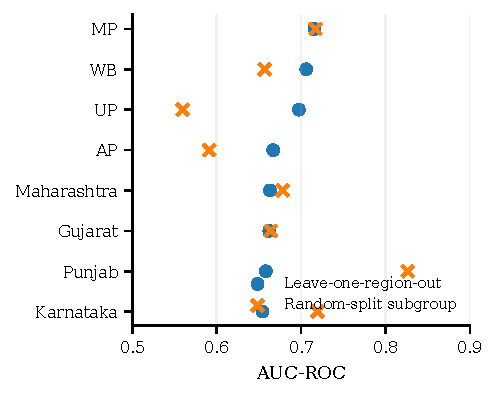
\includegraphics[width=\columnwidth]{fig_regional.pdf}
\caption{Leave-one-region-out $\auc$ (circles) against random-split subgroup $\auc$ for the same regions (crosses). Subgroup estimates on the random split are far more dispersed, reflecting small per-region test counts (142--238) rather than genuine heterogeneity in transferability.}
\label{fig:regional}
\end{figure}

Mean leave-one-region-out $\auc$ is $0.6781\pm0.0243$ (Table~\ref{tab:logo}), spanning 0.654 (Karnataka) to 0.716 (Madhya Pradesh). Figure~\ref{fig:regional} contrasts this with random-split subgroup performance, which ranges from 0.560 to 0.826 --- a far wider spread driven by per-region test counts of only 142--238. This contrast is itself a useful methodological point: subgroup metrics computed on a single split are dominated by sampling noise and should not be interpreted as regional performance without uncertainty quantification.

Regional prevalence on the random split ranges from 7.94\% to 16.81\%, and the maximum pairwise Wasserstein distance between regional predicted-PD distributions is 0.0716. We report no pass/fail fairness verdict. Region is not a protected attribute and is not an adequate proxy for caste, gender, land tenure, disability or any other dimension along which credit access disparity operates. A synthetic geographic stratum cannot support a fairness certification, and issuing one would be a category error.

We also disclose a limitation of this protocol: leave-one-region-out folds train on all other regions across \emph{all} dates, including dates after the held-out region's test records. Spatial transfer is therefore measured with temporal information leakage. A temporally blocked variant is left to future work.

\subsection{Decision-Analytic Sensitivity}

\begin{table}[!t]
\caption{Threshold Diagnostics, Random and Out-of-Time Test Sets}
\label{tab:threshold}
\centering
\footnotesize
\setlength{\tabcolsep}{4pt}
\begin{tabular}{@{}llccccc@{}}
\toprule
Split & $\tau$ & Flag & Sens. & Spec. & Prec. & Net benefit \\
\midrule
\multirow{6}{*}{Random}
 & 0.05 & 0.844 & 0.934 & 0.168 & 0.136 & 0.0766 \\
 & 0.10 & 0.503 & 0.721 & 0.527 & 0.176 & 0.0427 \\
 & 0.15 & 0.286 & 0.492 & 0.743 & 0.212 & 0.0208 \\
 & 0.20 & 0.151 & 0.299 & 0.870 & 0.244 & 0.0083 \\
 & 0.25 & 0.078 & 0.183 & 0.937 & 0.288 & 0.0040 \\
 & 0.30 & 0.046 & 0.127 & 0.965 & 0.338 & 0.0025 \\
\midrule
\multirow{6}{*}{OOT}
 & 0.05 & 0.860 & 0.958 & 0.159 & 0.181 & 0.1186 \\
 & 0.10 & 0.526 & 0.773 & 0.522 & 0.239 & 0.0811 \\
 & 0.15 & 0.302 & 0.581 & 0.752 & 0.313 & 0.0578 \\
 & 0.20 & 0.156 & 0.369 & 0.886 & 0.386 & 0.0361 \\
 & 0.25 & 0.084 & 0.204 & 0.939 & 0.393 & 0.0160 \\
 & 0.30 & 0.044 & 0.115 & 0.969 & 0.423 & 0.0078 \\
\bottomrule
\end{tabular}
\end{table}

\begin{figure*}[!t]
\centering
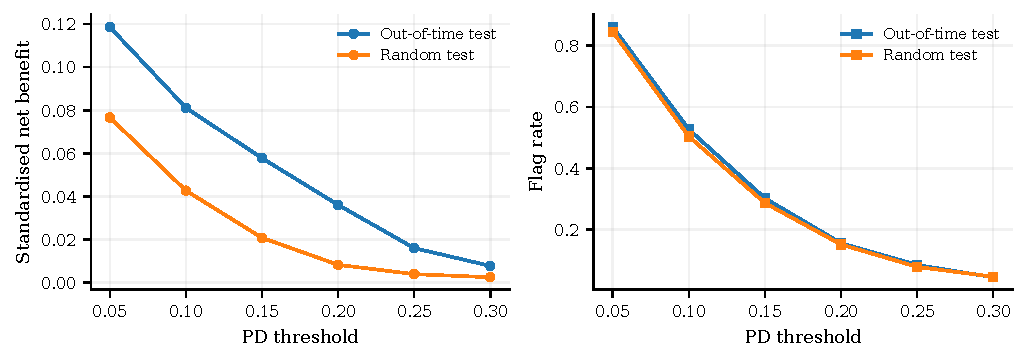
\includegraphics[width=0.85\textwidth]{fig_threshold.pdf}
\caption{Decision-curve analysis. Left: standardised net benefit against PD threshold. Right: flag rate against threshold. The two splits diverge substantially in net benefit at every threshold despite similar flag rates, because prevalence differs.}
\label{fig:threshold}
\end{figure*}

Table~\ref{tab:threshold} and Figure~\ref{fig:threshold} report six thresholds, following decision-curve methodology \cite{vickers2006decision}. At $\tau=0.15$ the flag rate is similar across splits (0.286 versus 0.302) but precision differs sharply (0.212 versus 0.313) and net benefit nearly triples (0.0208 versus 0.0578). A fixed threshold therefore implies materially different operating behaviour before and after the regime shift --- a decision rule calibrated on the earlier period would flag a similar fraction of applicants while the meaning of a flag changed substantially.

Net benefit here assumes unit benefit for identifying a default and a threshold-implied relative cost for false positives. It is not a profit estimate: it omits loan size, loss given default, recovery, and the welfare cost of denying credit to a borrower who would have repaid. These thresholds are diagnostic probes. None is a recommended policy.

\subsection{Score Transformation}
For communication only, we map PD to a points-to-double-the-odds score with anchor odds $O_\ast=19$ (i.e.\ anchor PD $=0.05$), anchor score $S_\ast=600$ and PDO $=40$:
\begin{equation}
S(p)=S_\ast-\frac{\text{PDO}}{\ln 2}\ln\!\left(\frac{p/(1-p)}{1/O_\ast}\right),
\label{eq:pdo}
\end{equation}
clipped to $[300,900]$. Thus $p=0.05\mapsto600$ and a doubling of bad odds costs exactly 40 points; the reproduction artifact should include unit tests at the six reported probabilities.

We deliberately publish \emph{no approval bands}. Band selection requires observed portfolio economics, affordability analysis, reject inference, calibration on real defaults and institutional governance approval, none of which a synthetic study can supply. Equation~\eqref{eq:pdo} is an interface, not a policy.

\subsection{Counterfactual Causal Interventions}
\label{sec:causal}
Sections~\ref{sec:stress}.1--\ref{sec:stress}.4 probe transfer across realised regimes of $\dgp$ (time, geography, threshold). Because $\dgp$ is fully specified in closed form, we can additionally perform \emph{structural interventions}: fix one covariate to a constant value for every record in an already-generated test cohort, hold every model exactly as fitted under the standard protocol of Section~\ref{sec:benchmark}, and re-score. This is a $do(\cdot)$-style counterfactual manipulation of a known generative process, not an observational subgroup comparison, and it isolates the sensitivity of each fitted model to one declared structural channel of \eqref{eq:drought}--\eqref{eq:latent}.

We evaluate two interventions on the same held-out test fold used elsewhere in Section~\ref{sec:stress}. The \emph{severity shock} sets $d_i=0.85$ for every record, an extreme, near-worst-case drought level, without altering any other covariate; because irrigation, soil moisture and NDVI are themselves downstream functions of $d_i$ in \eqref{eq:sm}--\eqref{eq:temp} at generation time, this intervention is applied to a freshly regenerated cohort under the constant-drought condition rather than by overwriting drought alone in the existing test records, so that the full downstream climate block reflects the shock consistently. The \emph{decoupling shock} instead sets $\text{irr}_i=0$ for every record, severing the drought-attenuation channel in \eqref{eq:drought} (the $-0.18\,\text{irr}_i$ term) so that drought exposure translates into downstream stress and, through $D_i$ and $C_i$, into default risk without the buffering effect of irrigation access.

\begin{table}[!t]
\caption{Counterfactual Stress Test: Change from Baseline at $\tau=0.15$}
\label{tab:causal}
\centering
\footnotesize
\setlength{\tabcolsep}{3.2pt}
\begin{tabular}{@{}llccc@{}}
\toprule
Model & Scenario & $\Delta\auc$ & $\Delta\text{ECE}_{10}$ & $\Delta\text{NB}_{0.15}$ \\
\midrule
\multirow{2}{*}{Logistic regression} & Severity  & $+0.0016$ & $+0.0046$ & $-0.0004$ \\
                                      & Decoupling& $+0.0035$ & $+0.0025$ & $+0.0013$ \\
\multirow{2}{*}{Random forest}       & Severity  & $-0.0033$ & $+0.0209$ & $-0.0061$ \\
                                      & Decoupling& $+0.0022$ & $-0.0020$ & $-0.0032$ \\
\multirow{2}{*}{Hist.\ boosting}     & Severity  & $-0.0071$ & $-0.0074$ & $-0.0019$ \\
                                      & Decoupling& $-0.0013$ & $-0.0011$ & $+0.0014$ \\
\multirow{2}{*}{XGBoost}             & Severity  & $-0.0007$ & $+0.0104$ & $-0.0054$ \\
                                      & Decoupling& $-0.0006$ & $-0.0013$ & $+0.0003$ \\
\bottomrule
\end{tabular}
\end{table}

\begin{figure}[!t]
\centering
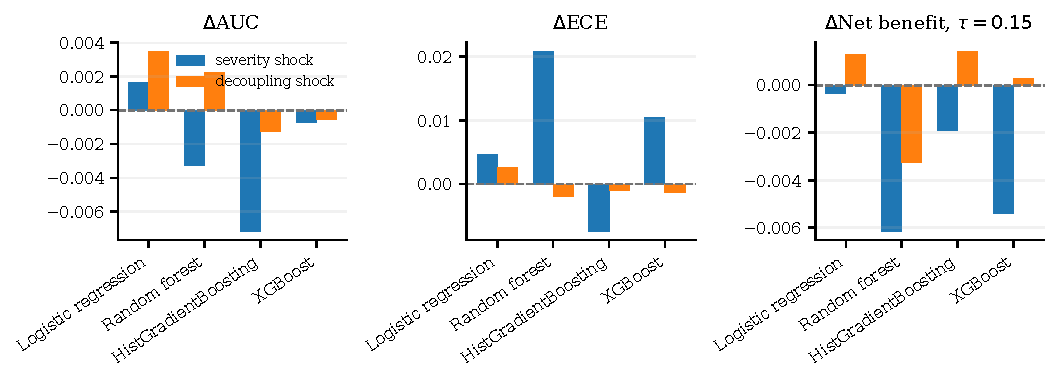
\includegraphics[width=\columnwidth]{fig_stress_test.pdf}
\caption{Counterfactual causal interventions. AUC, ECE and net benefit at $\tau=0.15$ under baseline, severity-shock ($\text{drought\_risk}=0.85$) and decoupling-shock ($\text{irrigation\_access}=0$) conditions, by model.}
\label{fig:causal}
\end{figure}

Table~\ref{tab:causal} and Figure~\ref{fig:causal} show that discrimination is close to invariant under both interventions for every model: the largest AUC movement is $-0.0071$ (HistGradientBoosting, severity shock), an order of magnitude smaller than the rolling-origin spread reported in Section~\ref{sec:stress}.2. Calibration is more sensitive: the severity shock raises ECE by up to $0.021$ (random forest) and $0.010$ (XGBoost), indicating that pushing drought to an extreme, off-distribution level degrades probability accuracy for tree ensembles more than it degrades ranking. Net benefit at $\tau=0.15$ falls under the severity shock for every non-linear learner (by $0.002$--$0.006$) but is essentially flat, or mildly positive, for logistic regression. The decoupling shock produces smaller and more mixed changes across all three metrics and all four models, consistent with irrigation access being a second-order attenuator of drought in \eqref{eq:drought} rather than the primary driver of $\eta_i$.

Two implications follow. First, because these are closed-form interventions on a known $\dgp$ rather than resampled data, the near-zero $\Delta\auc$ under an extreme drought condition is evidence that the fitted models are not simply detecting sample-composition shift, since composition is held fixed by construction of the intervention; the ranking sensitivity to $d_i$ itself is small under this generator's calibration. Second, the calibration degradation without matching discrimination loss reproduces, on a controlled synthetic counterfactual, the same discrimination/calibration dissociation documented empirically in Section~\ref{sec:stress}.1: a model can rank correctly under a shock to a structural channel while its predicted probabilities drift.

%=====================================================================
\section{Multi-Task Outcome Extensions}
\label{sec:multitask}
Requirement R7 (Section~\ref{sec:architecture}) attaches two supplementary targets, LGD in \eqref{eq:lgd} and Weibull time-to-default in \eqref{eq:weibull}, to the same point-in-time covariate vector used for the primary binary benchmark. This section reports baseline empirical performance on both, established with off-the-shelf estimators rather than a full model comparison, to demonstrate that the extension is usable, not to identify a best learner.

\subsection{Loss Given Default Regression}
We fit LGD only on defaulted records ($n=985$; 788 train, 197 test, an 80/20 split stratified as in Section~\ref{sec:benchmark}), regressing $\ell_i$ on the full 28-covariate vector with a standardised-feature ridge regressor ($\alpha=1$) and an XGBoost regressor (250 trees, depth 3, learning rate 0.04), clipping both models' predictions to $[0.05,0.95]$ to respect the support of \eqref{eq:lgd}.

\begin{table}[!t]
\caption{LGD Regression, Held-Out Test Fold ($n=197$)}
\label{tab:lgd}
\centering
\footnotesize
\begin{tabular}{@{}lcc@{}}
\toprule
Model & $R^2$ & MAE \\
\midrule
Ridge & \textbf{0.3771} & \textbf{0.0729} \\
XGBoost regressor & 0.3360 & 0.0750 \\
\bottomrule
\end{tabular}
\end{table}

Table~\ref{tab:lgd} shows ridge regression modestly outperforming the tuned XGBoost regressor on both $R^2$ (0.3771 versus 0.3360) and MAE (0.0729 versus 0.0750). This is consistent with \eqref{eq:lgd} being additive and near-linear in its declared covariates and Gaussian noise, so a linear learner needs no capacity for interaction terms that are not present in the generative mechanism; it should not be read as a general claim that linear models dominate LGD estimation on real portfolios, where nonlinear loss dynamics are well documented \cite{smaragdakis2021lgd}. Roughly 62--66\% of test-fold variance in $\ell_i$ is attributable to the idiosyncratic Gaussian term in \eqref{eq:lgd} and is therefore irreducible under either learner, by construction of the generator.

\subsection{Time-to-Default Survival Analysis}
We fit a penalised Cox proportional-hazards model ($\ell_2$ penalty, Newton-type optimisation of the partial likelihood) on standardised covariates, using the full 80/20 split ($n_{\text{train}}=6400$, $n_{\text{test}}=1600$) with $\delta_i$ as the event indicator and $T_i$ as the observed duration from \eqref{eq:weibull}. Discrimination is assessed with Harrell's concordance index \cite{harrell1982cindex}, computed on the linear risk score $\hat\eta_i=\mathbf{x}_i^\top\hat\beta$ against all comparable pairs in the held-out fold.

\begin{table}[!t]
\caption{Time-to-Default Survival Model, Held-Out Test Fold ($n=1600$)}
\label{tab:survival}
\centering
\footnotesize
\begin{tabular}{@{}lc@{}}
\toprule
Model & Harrell's $C$-index \\
\midrule
Cox proportional hazards (ridge) & 0.6093 \\
\bottomrule
\end{tabular}
\end{table}

Table~\ref{tab:survival} reports $C=0.6093$, meaningfully above the chance value of 0.5 \cite{cox1972regression,harrell1982cindex} but well short of the $\auc\approx0.67$--$0.71$ range reported for the binary outcome in Sections~\ref{sec:benchmark}--\ref{sec:stress}. This gap is expected rather than anomalous: the Weibull event time in \eqref{eq:weibull} is generated from the systematic risk index $\eta_i^{\text{sys}}$ alone, discarding the idiosyncratic term $\xi_i$ that contributes to the binary label, but the shape parameter $k=1.45$ and the independent uniform censoring process inject substantial additional variability into the observed duration $T_i$ that a linear risk score cannot recover.

\subsection{Implications for Benchmark Utility}
Both extensions attach directly to the existing covariate vector and split protocol, so a user of AgroScore can evaluate severity- and duration-aware quantitative risk models without modifying the primary classification benchmark or invalidating any previously reported number in Sections~\ref{sec:benchmark}--\ref{sec:stress}. The baseline results in Tables~\ref{tab:lgd} and~\ref{tab:survival} are intended as reference points for future comparisons, not as claims of production-grade LGD or survival modelling performance; as with the primary outcome, both targets remain closed-world constructs generated by a declared, non-estimated mechanism, and Sections~\ref{sec:threats}--\ref{sec:governance} apply to them without modification.

%=====================================================================
\section{Discussion}

\subsection{What the Benchmark Establishes}
Four findings are supported within the stated experimental scope.

\textbf{Model ranking depends on the outcome mechanism.} Logistic regression leads in the additive-logit reference regime, whereas tree ensembles lead in the threshold and conditional-interaction regimes. The original null result is therefore a specification-conditional sanity check, not evidence against nonlinear modelling. The near-tie in the hybrid regime also shows that adding nonlinear terms does not automatically create a material ensemble advantage.

\textbf{Financial history dominates climate information in the specified generator.} The financial block's ablation effect is $15\times$ the climate block's and is the only one stable across all ten seeds. The replicated learning curve shows no emerging climate advantage through $n=32\,000$, but does not by itself rule out sample-size effects under other generator settings.

\textbf{The engineered interaction shows no incremental benefit.} Despite entering the outcome model with a coefficient of 0.85, the evaluated ablation finds no measurable gain from supplying the compound feature once its components are present. This is a bounded negative result: an explicit composite of available variables is not necessarily incrementally informative under the evaluated learners and sample sizes.

\textbf{Discrimination and calibration dissociate under shift.} Out-of-time $\auc$ rises by 0.041 while ECE triples and the calibration intercept flips sign. Any evaluation reporting a single ranking metric would have concluded that the model transferred well.

\subsection{What It Does Not Establish}
The benchmark cannot speak to real-world accuracy. A synthetic label generated from modelled covariates is a closed world where the analyst fixes the answer. It cannot reproduce strategic borrower behaviour, loan restructuring, censoring, policy change, measurement error, missing-not-at-random satellite retrievals, spatial autocorrelation, or institution-specific underwriting overlays. Our metrics assess selected implementation and experimental-design properties; they estimate no benefit to any lender or farmer.

The relationship between our negative climate finding and the mixed empirical literature should be stated carefully. Our result is consistent with M\"ollmann \textit{et al.} \cite{mollmann2020vegetation}, but consistency is not corroboration: our generator was specified by us, and we chose how strongly climate enters the outcome. We report the finding as a property of a published process, not as evidence about Indian agriculture.

\subsection{Implications for Synthetic Data Practice}
\label{sec:governance}
Our broader claim is procedural. Downstream conclusions from synthetic data inherit defects in the generator, so generator descriptions should be accompanied by targeted diagnostics. The six tests in Section~\ref{sec:fidelity} are inexpensive and require no reference data, but each has limited power and addresses only a subset of possible failures. We propose them as a candidate minimum diagnostic set, supplemented by parameter, moment and conditional-distribution unit tests. Marginal direction checks and parameter-provenance disclosure (Table~\ref{tab:params}) are especially natural for mechanistic generators.

Finally, the governance boundary. Equation~\eqref{eq:pdo} satisfies its anchor and monotonicity tests, but a lender deploying anything resembling this pipeline would still require observed-default calibration, reject inference, capacity-to-pay constraints, stability monitoring, documented override procedures and independent model validation. Technical performance is one component of risk management \cite{nist2023airmf}, and on the evidence assembled here it is not the binding one.

%=====================================================================
\section{Threats to Validity}
\label{sec:threats}

\textbf{Construct validity.} The simulated default flag approximates a binary performance outcome and does not model delinquency duration, restructuring, recovery or exposure at default. NDVI and soil variables are stylised signals with plausible support and dependence, not extracted pixels; no MODIS granule was retrieved. The dataset tests code and estimator behaviour, not sensor validity.

\textbf{Internal validity.} Deterministic generation and point-in-time construction limit accidental leakage, but the results remain partly circular: covariates generate the label. The prespecified outcome-mechanism suite exposes sensitivity to this choice but cannot eliminate it. Hyperparameters are fixed rather than selected by nested cross-validation, which aids auditability but does not estimate each learner's attainable ceiling. The leave-one-region-out protocol mixes time periods, as disclosed in Section~\ref{sec:stress}.

\textbf{External validity.} Regional parameters are ordinally anchored to the Agriculture Census 2015--16 \cite{agcensus2016} but not fitted to it; only the ranking, not the magnitude, is literature-consistent (Table~\ref{tab:params}). The 30-day month convention makes simulated calendar years unequal (1\,761 records in 2019 versus 1\,412 in a truncated 2023), which affects rolling-origin sample sizes. MODIS pixels at 250\,m would mix multiple smallholdings in most of the modelled regions, and a 16-day composite may not align with underwriting dates. API latency, cloud contamination, field-boundary error, non-random missingness and changing agronomic practice are not represented at all.

\textbf{Statistical validity.} We report many comparisons: 7 models $\times$ 8 metrics, 6 pairwise contrasts, 5 ablations $\times$ 10 seeds, 3 rolling cuts, 8 regional folds and 6 thresholds. We apply no family-wise correction and therefore do not treat any individual nominal significance as confirmatory. Bootstrap intervals quantify test-set sampling variability conditional on the generated cohort and modelling protocol; they do not include generator-parameter uncertainty. The two-sample detector is model-specific rather than an equivalence test, and the distance ratio depends on scaling and metric choice. We therefore reserve stronger claims for effects that are stable across seeds or whose intervals are separated materially from zero.

\textbf{Decision validity.} Threshold metrics omit loan size, profit, loss given default, approval elasticity and the welfare cost of exclusion. Regional diagnostics are not, and cannot be, a fairness assessment.

%=====================================================================
\section{Protocol for External Validation}

Before any operational consideration, a follow-on study should: (1) preregister prediction timestamp, outcome window and default definition; (2) obtain consented longitudinal outcomes with documented lawful basis; (3) assemble every covariate strictly as known at prediction time, with versioned satellite products and explicit missingness rules; (4) group repeated loans by borrower and household to prevent within-entity leakage; (5) preserve an institutionally and temporally independent test set; (6) quantify satellite coverage, cloud contamination, retrieval missingness and drift; (7) assess calibration separately by crop, season, geography and relevant protected or vulnerable groups; (8) benchmark against both the lender's incumbent policy and a parsimonious scorecard, given the findings of Section~\ref{sec:benchmark}; (9) conduct cost, capacity-to-pay and decision-curve analysis with realistic loss given default; and (10) complete legal, privacy, security and model-risk review. Access to finance matters for smallholder development, but that objective does not lower the evidentiary bar for automated credit decisions --- if anything it raises it, since the cost of wrongful exclusion falls on those with fewest alternatives.

%=====================================================================
\section{Conclusion}

We presented AgroScore, a fully specified synthetic benchmarking framework for privacy-restricted agricultural credit research, together with six diagnostics adapted to the no-reference setting: two-sample detection testing ($\auc=0.5019\pm0.0042$), a cross-cohort near-duplicate check (DCR ratio $0.9956$), marginal directional agreement (10/10), spectral inspection (PC1 $=19.6\%$), a random-embedding moment distance of $0.1095$ between independently seeded cohorts, and attribution-to-mechanism rank conformance ($\rho=0.4592$ for XGBoost, $\rho=0.3861$ for HistGradientBoosting). These tests provide bounded evidence about implementation behaviour and should complement, not replace, parameter-level unit tests and validation against real data. We also demonstrated two multi-task outcome extensions --- LGD regression ($R^2=0.3771$, ridge) and Weibull time-to-default survival analysis ($C=0.6093$, Cox proportional hazards) --- attached to the same covariate vector and split protocol as the primary benchmark.

The four-regime experiment rejects a universal model-complexity conclusion. Logistic regression leads in the additive-logit reference regime, random forest under thresholds, histogram boosting under conditional interactions, and extra trees narrowly in the hybrid regime. The detailed reference-regime analysis remains useful as a recovery check: the stack is effectively tied with logistic regression, the financial-block ablation is the largest and most stable, and the engineered climate--debt feature has no measurable incremental benefit. Out-of-time evaluation raises $\auc$ to 0.712 while tripling expected calibration error and flipping the calibration intercept from $-0.392$ to $+0.437$, demonstrating that ranking and probability accuracy can dissociate under shift.

The benchmark is intended for methodological comparison, software testing, teaching and protocol development. It is not evidence of lending utility, and the resulting score must not be used to approve, price or decline credit. Establishing utility requires prospectively timestamped, consented longitudinal outcomes and independent governance review.

%=====================================================================
\section*{Reproducibility, Ethics and Declarations}

\textbf{Code and data availability.} The exact generator and analysis implementation used for this manuscript, figure scripts, pinned dependencies, the synthetic cohort, held-out predictions for every model and split, and the machine-readable results underlying the tables and figures are archived at \url{https://doi.org/10.5281/zenodo.22871548}. All reported results regenerate from seed 20260916. The author is responsible for verifying, immediately before submission, that the archived contents are byte-identical to the code that produced the numbers in this manuscript; an archive that drifts from the reported numbers after this point is a reproducibility failure regardless of the DOI's validity.

\textbf{Ethics.} Every record is synthetic. No human participants, borrower records or real credit decisions were involved, and no institutional data were accessed. Future work on borrower data must obtain appropriate ethical approval and data-use authorisation.

\textbf{Funding.} No external funding. \textbf{Competing interests.} None declared.

\textbf{Use restriction.} The software, models and scores are research artifacts. They must not be used to approve, price or decline credit, or be represented as validated for any lending purpose.

\balance
\bibliographystyle{IEEEtran}
\bibliography{agroscore,agroscore_additions}

\begin{IEEEbiographynophoto}{Aastik Srivastava}
is an undergraduate student at the Manipal Institute of Technology, Manipal Academy of Higher Education, Manipal, India. His research interests include applied machine learning, credit risk modelling, remote sensing for development applications, and reproducible research methodology.
\end{IEEEbiographynophoto}

\end{document}
